\documentclass{ATLAS_latex/atlasnote} 
\skipbeforetitle{-5pt}

\usepackage{graphicx,multirow}
\usepackage{epstopdf}
\usepackage{authblk}
\usepackage{hyperref}
\usepackage{pdfpages,subfigure,caption,placeins}
\usepackage{color}

\newcommand{\red}[1]{\textcolor[rgb]{1,0,0}{#1}}

%\newcommand{\et}{\mbox{$E_{T}$}}
%\newcommand{\met}{\mbox{$\protect \raisebox{.3ex}{$\not$}\et$}}
%\newcommand{\ppbar}{\mbox{$p\overline{p} \ $}}
\newcommand{\pbarp}{\mbox{$\overline{p}p$}}
\newcommand{\hs}{\hspace*{0.375in}}
\newcommand{\zmumu}{\mbox{$Z \rightarrow \mu\mu$}}
\newcommand{\zee}{\mbox{$Z \rightarrow ee$}}
\newcommand{\psimumu}{\mbox{J/$\psi \rightarrow \mu\mu$}}
\newcommand{\oopsmumu}{\mbox{$\Upsilon \rightarrow \mu\mu$}}
%\newcommand{\mtop}{\mbox{$M_{top}$}}
\newcommand{\pt}{\mbox{P_{T}}}
\newcommand{\topq}{\mbox{${\rm top-quark}$}}
\newcommand{\topdecaylj}{$ \overline{t}$}
%\newcommand{\tt}{$ t \bar t$}
%\newcommand{\ttbar}{$t\bar{t} \ $}
\hyphenation{posi-trons in-di-rect-ly mod-el-ling}

%
% Input some definitions
%
%
%----------  PHYSICS COMMANDS
%
\def \Et {{\rm E}_{\rm T}}
\def \Pt {{\rm P}_{\rm T}}
\def \Pz {{\rm P}_{\rm Z}}
\def \enu {\epsilon_{\nu}}
\def \stw {$\sin^{2}\theta_{W}$}
\newcommand{\MET}{\mbox{$\protect \raisebox{.3ex}{$\not$}\et$}}
\newcommand{\METC}{\mbox{$\protect \raisebox{.3ex}{$\not$}\etc$}}
%\def \MET {\not\!\Et}
\def\deg{^\circ}
\def\qbar{{\bar q}}
\def\nubar{{\bar \nu}}
\def\W{{\em W\/ }}
\def\Z0{${\em Z^0\/}$}
\def \lum {{\cal L}}
\def\epem{{\rm e^{+}e^{-}}}
\def\tptm{{\tau^{+}\tau^{-}}}
\def\roots{${\sqrt s}\:$}
\def\r#1 {$^{#1}$}
\def\sigW {$\sigma\cdot$B(\W$\rightarrow~$e $\nu$) }
\def\sigZ {$\sigma\cdot$B(\Z0$\rightarrow~\epem$) }
\hyphenation{brem-sstrah-lung proc-ess}
%
\def\first{{\mbox{$I\leq$}4~GeV}}
\def\second{{QC=\mbox{$I\leq$}~4~GeV+\mbox{$s_{ip}\leq$}~4}}
\def\third{{QC+\mbox{$\delta \phi \geq 2$}}}
\def\fourth{{QC+\mbox{$|\cos \theta^{*}| \leq 0.4$}}}
\def\fifth{{QC+\mbox{$\delta \phi \geq 2$}+\mbox{$|\cos \theta^{*}|\leq 0.4$}}} 
\def\six{{QC+\mbox{$\sum p_t  \leq$}40~GeV+\mbox{$\sum s_{ip} \leq 30$}}}
\def\seven{{\mbox{$\delta \phi \geq 2$}}}
\def\eight{{\mbox{$|\cos \theta^{*}| \leq 0.4$}}}
\def\nine{{\mbox{$\delta \phi \geq 2$}+\mbox{$|\cos \theta^{*}| \leq 0.4$}}} 
%
%\input moredefs.tex
%
%
%
%
\newcommand{\etc}{{\rm E}_{\scriptscriptstyle\rm T}^{\scriptscriptstyle\rm C}}
\newcommand{\et}{{\rm E}_{\scriptscriptstyle\rm T}}
\newcommand{\etcone}{{\rm E}_{\scriptscriptstyle\rm T}^{cone}}
\newcommand{\abseta}{\mid \eta^{det} \mid \leq}
\newcommand{\abz}{\mid z \mid \leq}
\newcommand{\fb}{f_{b}}
\newcommand{\ks}{K_{s}^{0}}
\newcommand{\pich}{\pi^{\pm}}
\newcommand{\piz}{ \pi^{0} }
\newcommand{\bigz}{{\cal Z}}
\newcommand{\emf}{f_{em}}
\newcommand{\deltar}{\sqrt{\Delta \eta ^{2}+ \Delta \phi ^{2}}}
\newcommand{\etprime}{{\rm E}_{\scriptscriptstyle\rm T'}}
\newcommand{\ptran}{{\rm P}_{\scriptscriptstyle\rm T}}
\newcommand{\met}{\mbox{$\protect \raisebox{.3ex}{$\not$}\et \ $}}
\newcommand{\wenu}{W \rightarrow e \nu}
\newcommand{\wmunu}{W \rightarrow \mu \nu}
\newcommand{\wlep}{W \rightarrow \rm{lepton}\, \nu}
\newcommand{\zv}{{\rm z}_{vertex}}
\newcommand{\wbb} {W b\bar{b} }
\newcommand{\wcc} {W c\bar{c} }
\newcommand{\ppbar}{p\bar{p}}
\newcommand{\qqbar}{q\bar{q}}
\newcommand{\ttbar}{t\bar{t}}
\newcommand{\bbbar}{b\bar{b}}
\newcommand{\ccbar}{c\bar{c}}
\newcommand{\ppbb} { \ppbar \rightarrow  \bbbar }
%\newcommand{\zee}{Z \rightarrow e^{+}e^{-} }
\newcommand{\bele}{b \rightarrow c e \nu_{e} }         
\newcommand{\blnu}{b \rightarrow c l \nu_{l} }         
\newcommand{\mtran}{{\rm M}_{\scriptscriptstyle\rm T}}
\newcommand{\acceff}{\rm{A} \times \epsilon}
\newcommand{\bbar} {\bar{b}}   
\newcommand{\gbb} { g \rightarrow b\bar{b} }
\newcommand{\gcc} { g \rightarrow c\bar{c}}
\newcommand{\tbar} { \bar{{t}}  }                                
\newcommand{\Lik}{\mbox{$\mathcal{L}$ }}
\newcommand{\Ki}{\mbox{$\chi^{2}$ }}
\newcommand{\mPr}{\mathcal{P}}
\newcommand{\CPr}{\mbox{$\mathcal{C}$ }}
\newcommand{\mLik}{\mathcal{L}}
\newcommand{\mCPr}{\mathcal{C}}
% dilepton symbols1
\def \mc {\multicolumn}
\def \pb    {pb$^{-1} $}
\def \DeltaPhi {$\Delta \phi_{\ell\,\ell \ }$} 
\def \mtop {$M_{top} \ $}
\def \mtopev {$M_{top}^{event} $}
\def \mw {$M_{W} \ $}
\def \ztau   {$Z\rightarrow\tau\tau \:$}
\def \DeltaPhil {$\Delta \phi{(\MET,\ell) \ }$} 
\def \DeltaPhij {$\Delta \phi{(\MET,j) \ }$} 
\def \TTbar {$t\overline{t} \; \;$}
\def \dpemu {\Delta \phi_{e\mu}}
\def \Mt {M_{top}}
\def \mtenu  {M_{T}^{e\nu}}
\def \lum {\cal L}
\def \intlum {\int {\cal L} dt}
\def \Zee {Z^{0} \rightarrow e^{+}e^{-}}
\def \Zmumu {Z^{0} \rightarrow \mu^{+}\mu^{-}}
\def \emu {e \mu}  
\def \temux {\ttbar \rightarrow \emu + X}
\def \tljx {\ttbar \rightarrow \ell \nu q \bar{q}^{\prime} b \bar{b} X}
\def \tllx {\ttbar \rightarrow \ell^+ \bar{\nu} \ell^- \nu b \bar{b} X}
\def \thad {\ttbar \rightarrow q \bar{q} b q \bar{q} \bar{b} X}   
\def \Ete {E_T^{e}}
\def \Ptmin {P_T^{min}}
\def \Ptmu {P_T^{\mu}}
\def \Etmiss {{\not}{E_T}}
% end of dilepton
%---------- UNITS, SYMBOLS
%
\newcommand{\imb}{ \mu {\rm b}^{-1} }
\newcommand{\inb}{ {\rm nb}^{-1} }
\newcommand{\ipb}{ {\rm pb}^{-1} }
\newcommand{\degs}{\mbox{$^{\circ}$}}
\newcommand{\gsim}{\mbox{\small$\stackrel{>}{\sim}$\normalsize}}
\newcommand{\lsim}{\mbox{\small$\stackrel{<}{\sim}$\normalsize}}
\newcommand{\gev}  { {\rm GeV}}
\newcommand{\tev}  { {\rm TeV}}
\newcommand{\gevc} { {\rm GeV/c}}
\newcommand{\gevcc}{ {\rm GeV/c^2}}

%
%---------- TYPE SETTING
%
\newcommand{\etal}{{\em et al.}}
\newcommand{\tableskip}{\vskip 5pt plus3pt minus1pt \relax}
\newcommand{\tindent}{\hskip 17pt}
\newcommand{\hfull}{\hspace*{\fill}}
\newcommand{\tline}{\protect\linebreak[4]\hfull}
\newcommand{\linespace}[1]{\protect\renewcommand{\baselinestretch}{#1}
  \footnotesize\normalsize}
%
%---------- Journal names
%
%\newcommand{\prl}[1]{Phys. Rev. Lett {\bf #1}}
%\newcommand{\prev}[1]{Phys. Rev. {\bf #1}}
%\newcommand{\prd}[1]{Phys. Rev. D {\bf #1}}
%\newcommand{\zs}[1]{Z. Phys. {\bf #1}}
%\newcommand{\ncim}[1]{Nuovo Cim. {\bf #1}}
%\newcommand{\plet}[1]{Phys. Lett. {\bf #1}}
%\newcommand{\prep}[1]{Phys. Rep. {\bf #1}}
%\newcommand{\rmp}[1]{Rev. Mod. Phys. {\bf #1}}
%\newcommand{\nphy}[1]{Nucl. Phys. {\bf #1}}
%\newcommand{\nim}[1]{Nucl. Instrumen. Meth. {\bf #1}}
%

%------------- Figure commands and macros
%
%
%  Called the same way epsffile is called.  Difference is it will center
%  the graphic in the page useing the center environment.
%
\def\gepsfcentered#1{
  \def\testit{#1}
  \def\lbracket{[}
  \ifx\testit\lbracket
    \let\dofilecmd=\gepsfwithopt
  \else
    \let\dofilecmd=\gepsfnoopt
  \fi
  \dofilecmd}

\def\gepsfnoopt#1{
  \begin{center}
  \leavevmode
  \epsffile{#1}
  \end{center}}

\def\gepsfwithopt#1 #2 #3 #4]#5{
  \begin{center}
  \leavevmode
  \gepsfmaxx=0.94\textwidth
  \epsffile[#1 #2 #3 #4]{#5}
  \end{center}}

%
%  Auto sizing for epsf figures that are larger than the text width.
%
\newdimen\gepsfmaxx
\gepsfmaxx=0.94\textwidth
\def\epsfsize#1#2{
  \ifnum \epsfxsize=0
    \ifnum \epsfysize=0
      \ifnum #1 > \gepsfmaxx
        \gepsfmaxx
	%\message{Did scaling.}
      \else
        #1
	%\messaeg{Used nat scaling}
      \fi
    \else
      \epsfxsize
      %\message{Using what ever.}
    \fi
  \else
    \epsfxsize
    %\message{Again, using whatever.}
  \fi
  %\message{Hi epsfxsize is \the\epsfxsize ...}
  %\message{epsfysize is \the\epsfysize ...}
  %\message{Hi first arg is \the#1 ...}
  %\message{Second arg is \the#2 ...}
}


\renewcommand{\topfraction}{0.95}
\renewcommand{\bottomfraction}{0.8}
\renewcommand{\textfraction}{0.06}
\renewcommand{\floatpagefraction}{0.85}
\setcounter{totalnumber}{5}
\setcounter{topnumber}{4}

\bibliographystyle{apsrev}

\title {Simple Simulation of the Micromegas Trigger at High Rates, and a Proposal for Improving the $\phi$ Measurement}

\usepackage{authblk}
\renewcommand\Authands{, } % avoid ``. and'' for last author
\renewcommand\Affilfont{\itshape\small} % affiliation formatting
\author[a,b]{J.~Farah}
\author[a]{N.~Felt}
\author[a]{M.~Franklin}
\author[a]{P.~Giromini}
\author[a]{J.~Philion}
\author[a]{A.~Tuna}
\author[a]{A.~Wang}
\affil[a]{Harvard University, Cambridge, Massachusetts 02138, USA}
\affil[b]{University of Massachusetts Boston, Boston, Massachusetts 02125, USA}

\abstracttext{\noindent We simulated the MM Trigger Processor at high rates. We can improve the non-precision measurement dramatically.}

\clearpage

\begin{document} 

\setcounter{page}{2}

\section{Introduction}
\label{sec:intro}

Introduction.



\section{Micromegas detector and electronics}
\label{sec:experiment}

Micromegas detector and electronics.

Test stand measurements.

\begin{figure}[!htpb]
  \begin{center}
    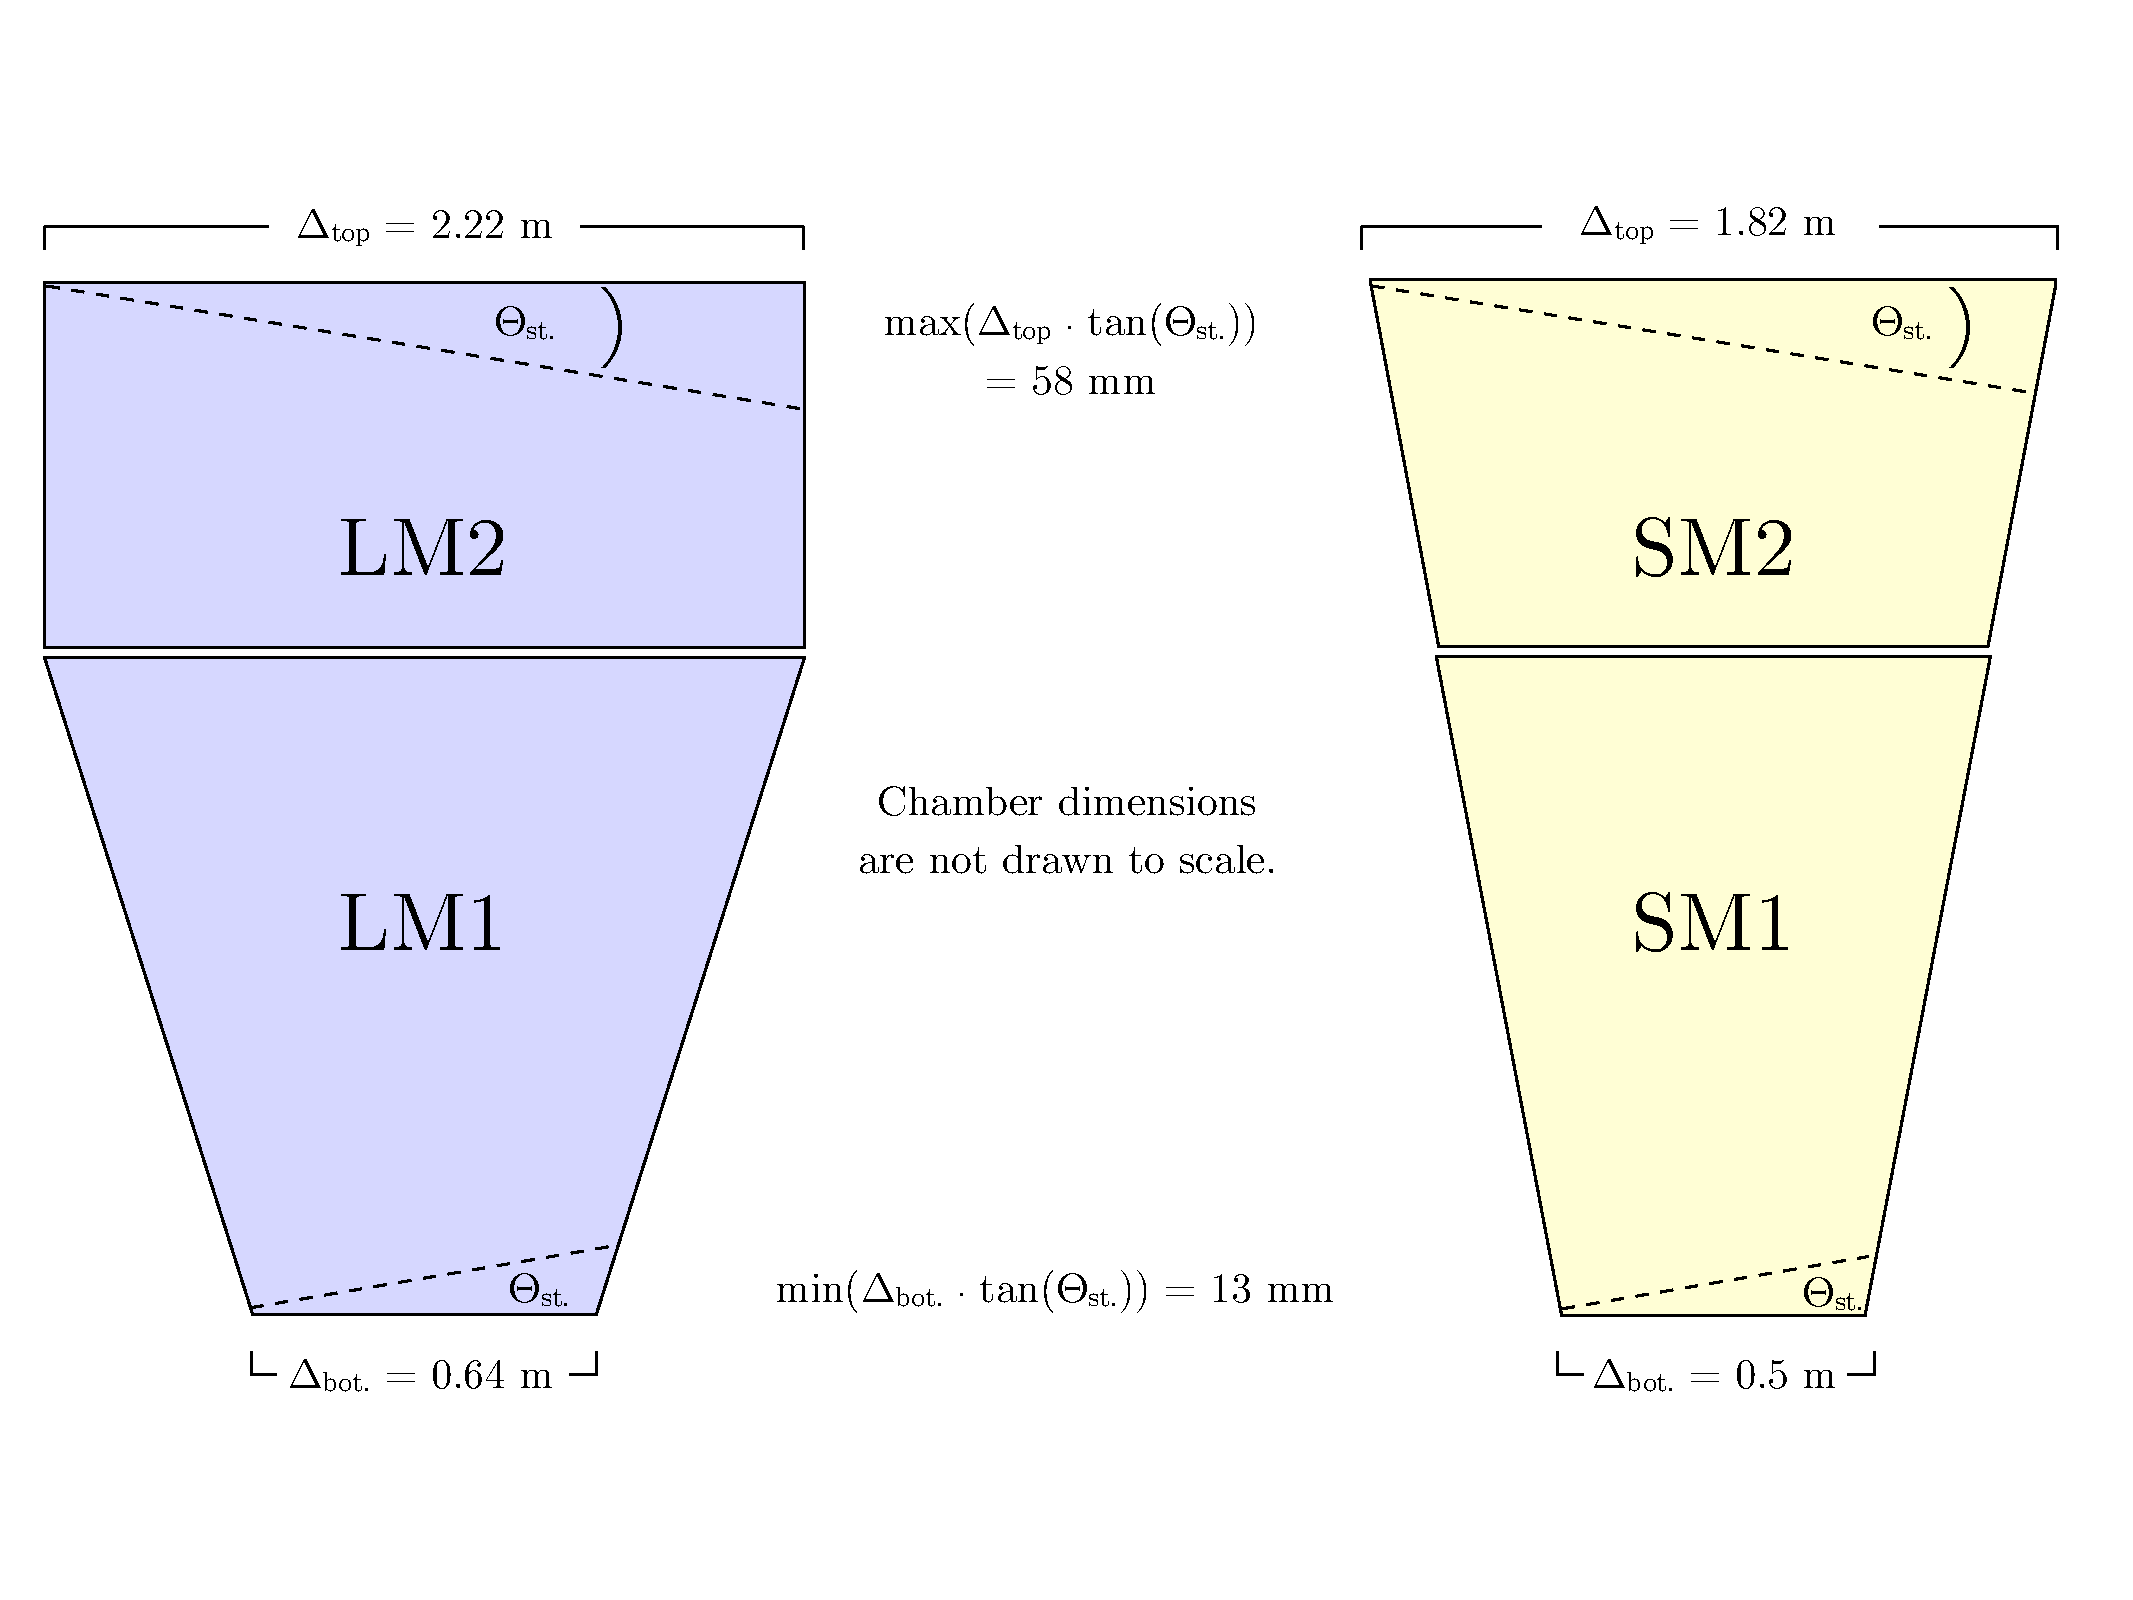
\includegraphics[width=0.9\textwidth]{figures/cartoon_chambers.pdf}
  \end{center}
  \vspace{-10pt}
  \caption{Drawings of Micromegas wedges with dimensions as specified by the NSW TDR. The stereo strips require larger roads than the horizontal strips because they overlap a band of $x$ strips of width from 13 to 58 mm.}
  \label{fig:chambers}
\end{figure}


\section{High luminosity LHC}
\label{sec:hllhc}

HL-LHC conditions.


\section{Simulation}
\label{sec:sim}

Standalone simulation.



\section{Nominal algorithm}
\label{sec:nominal}

Nominal algorithm and performance.

\begin{figure}[!htpb]
  \begin{center}
    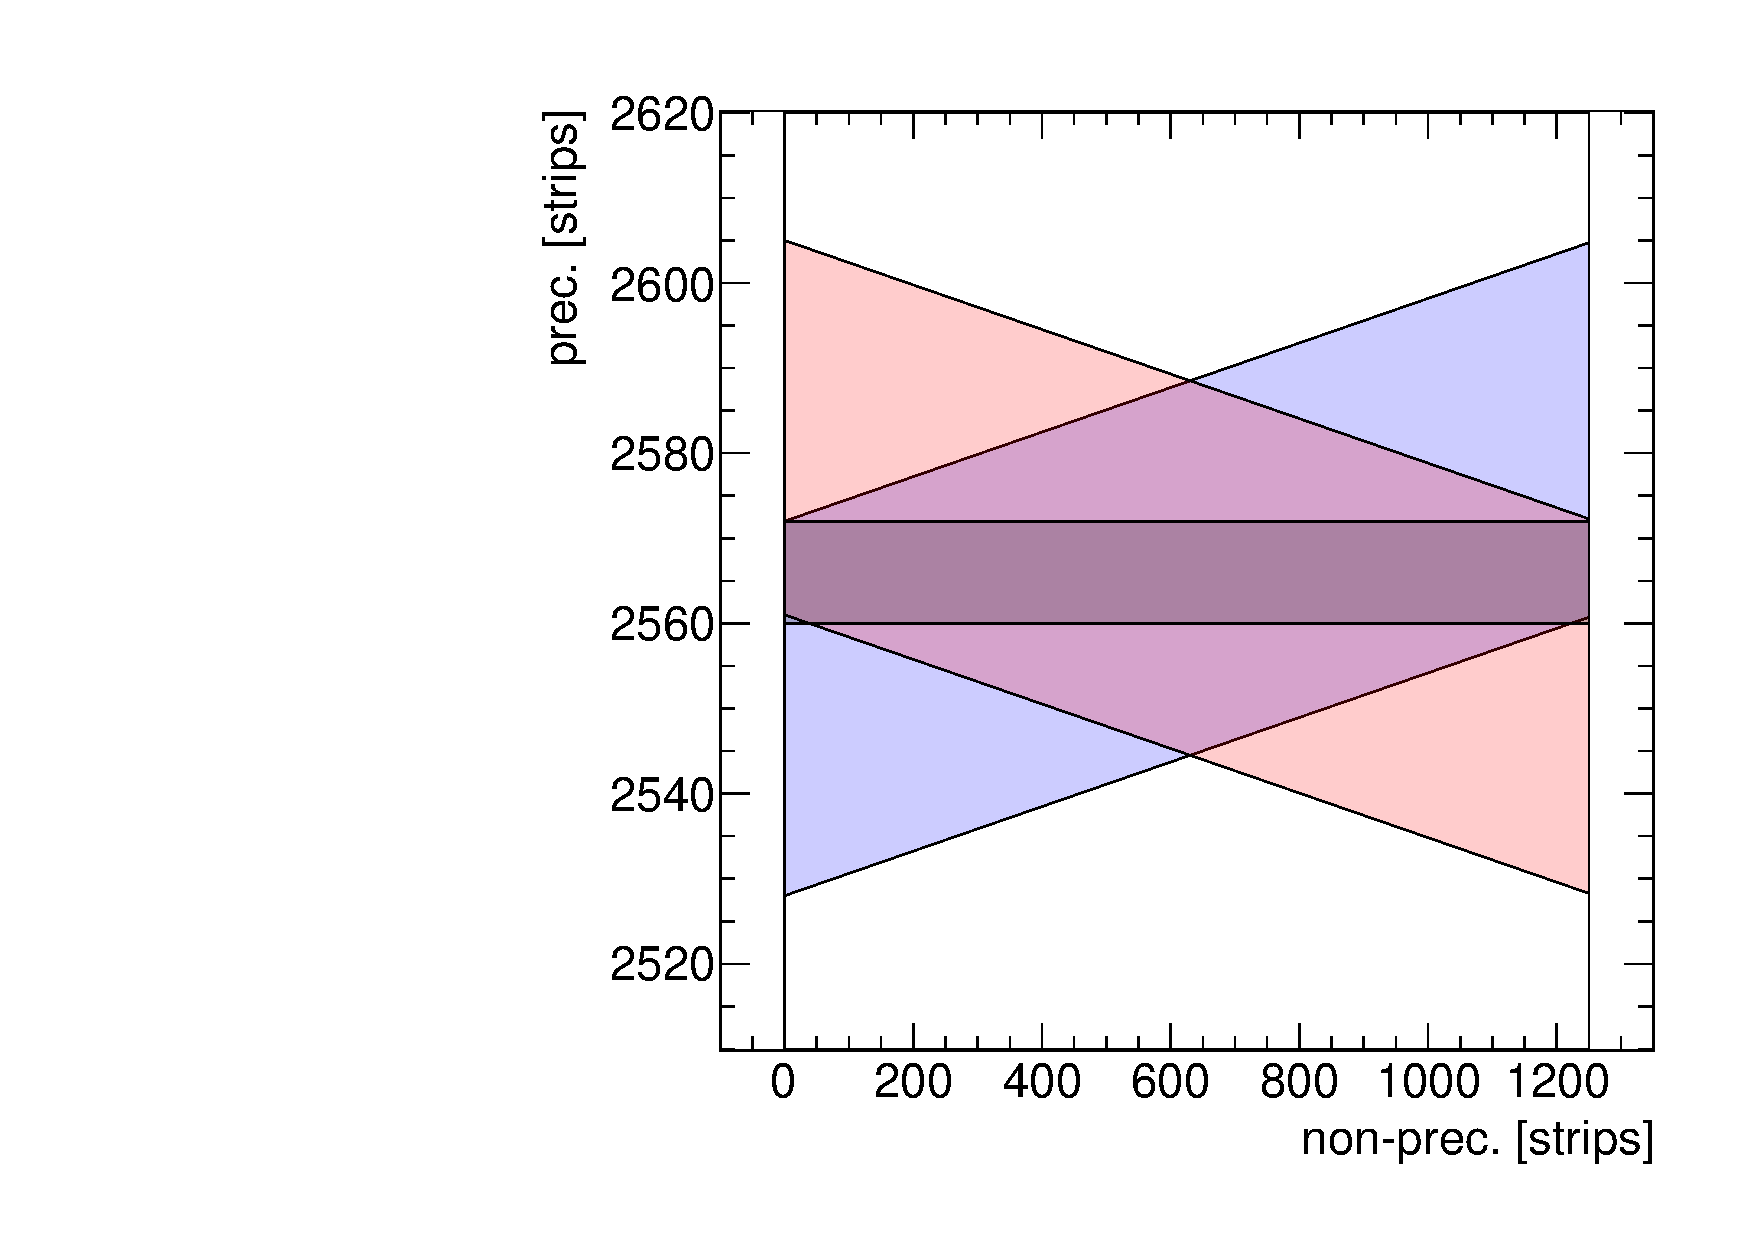
\includegraphics[width=0.48\textwidth]{figures/cartoon_roads_small_nominal.pdf}
    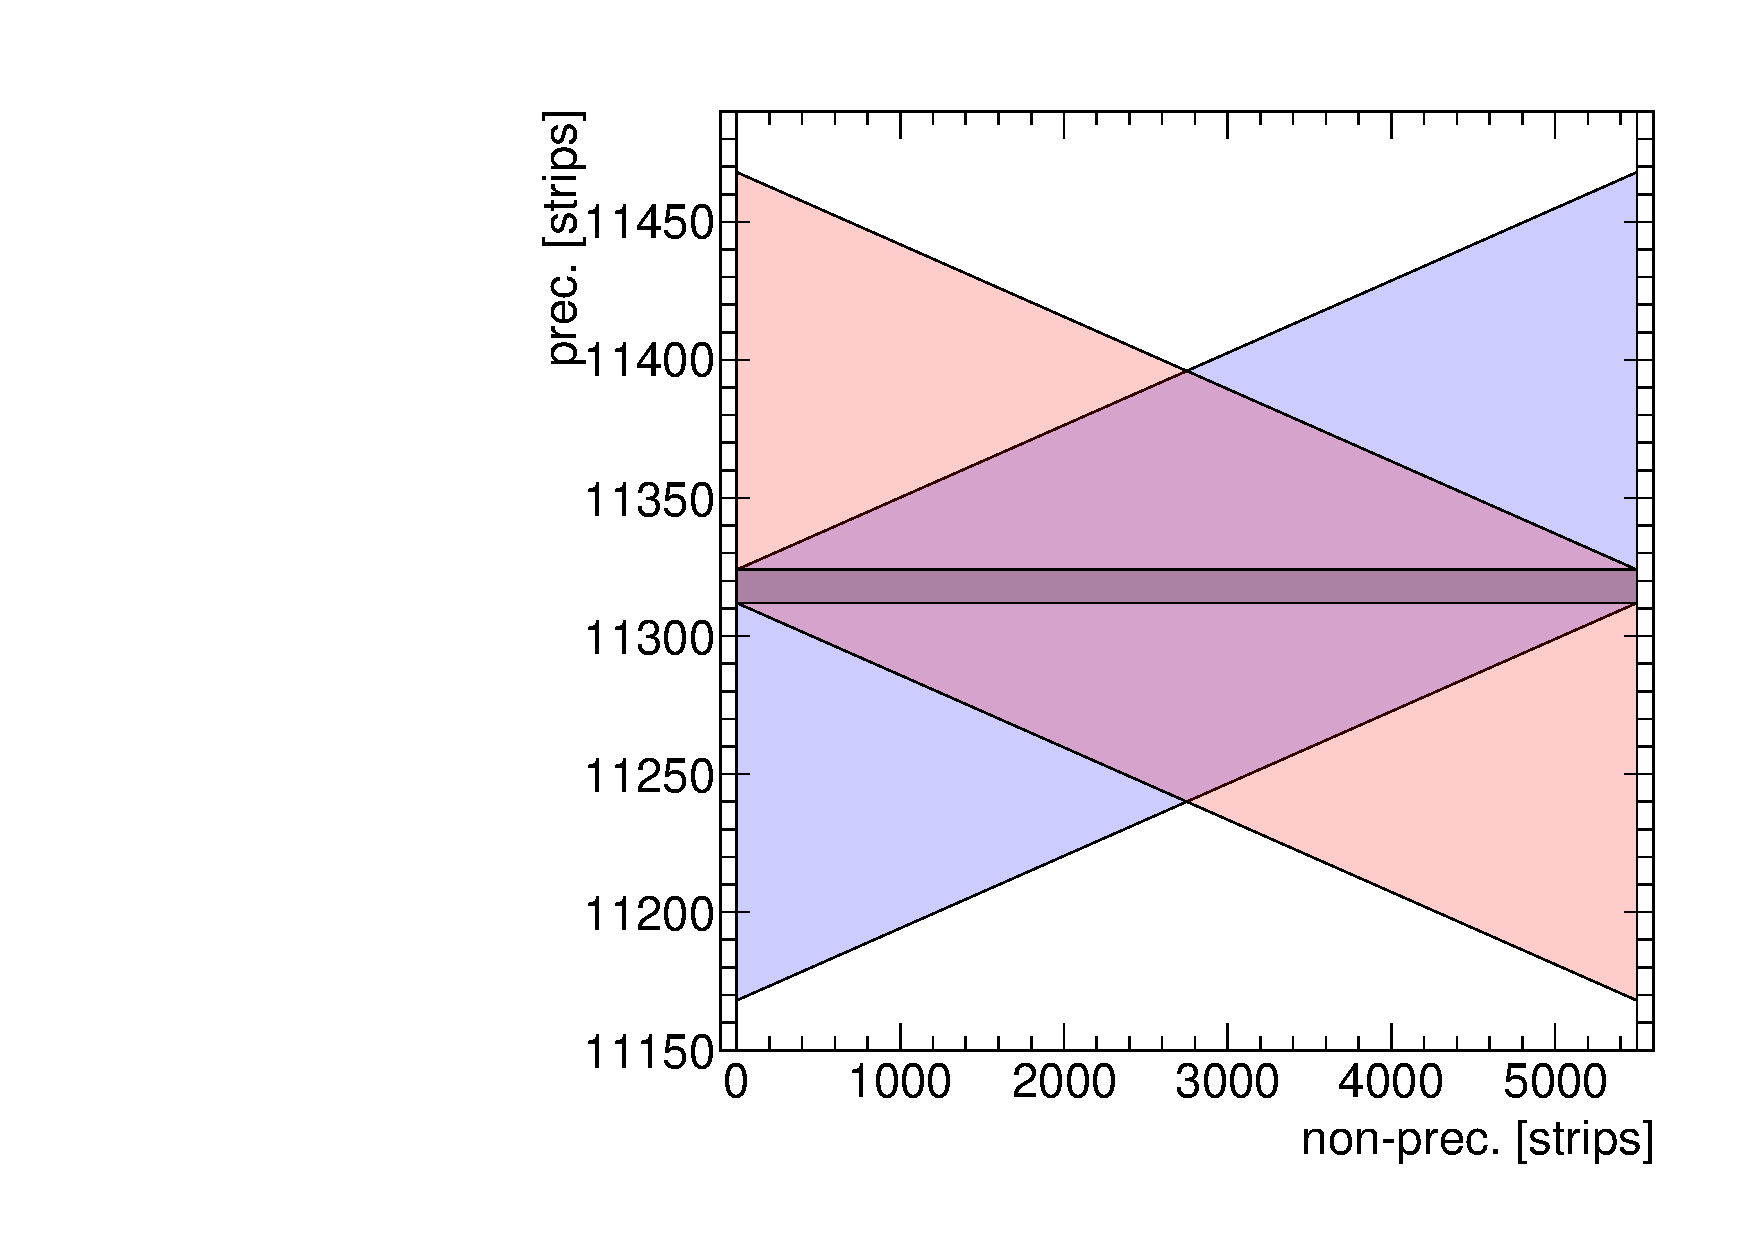
\includegraphics[width=0.48\textwidth]{figures/cartoon_roads_large_nominal.pdf}
  \end{center}
  \vspace{-10pt}
  \caption{Sketch of the road coverage of the nominal MMTP algorithm, for a small chamber closest to the beamline (left) and large chamber farthest from the beamline (right). The $X$ road is horizontal, the $U$ road is pink and slanted, and the $V$ road is blue and slanted. The x-axis and y-axis are in units of strip pitches, which are 0.4 mm.}
  \label{fig:cartoon_nominal}
\end{figure}

\begin{figure}[!htpb]
  \begin{center}
    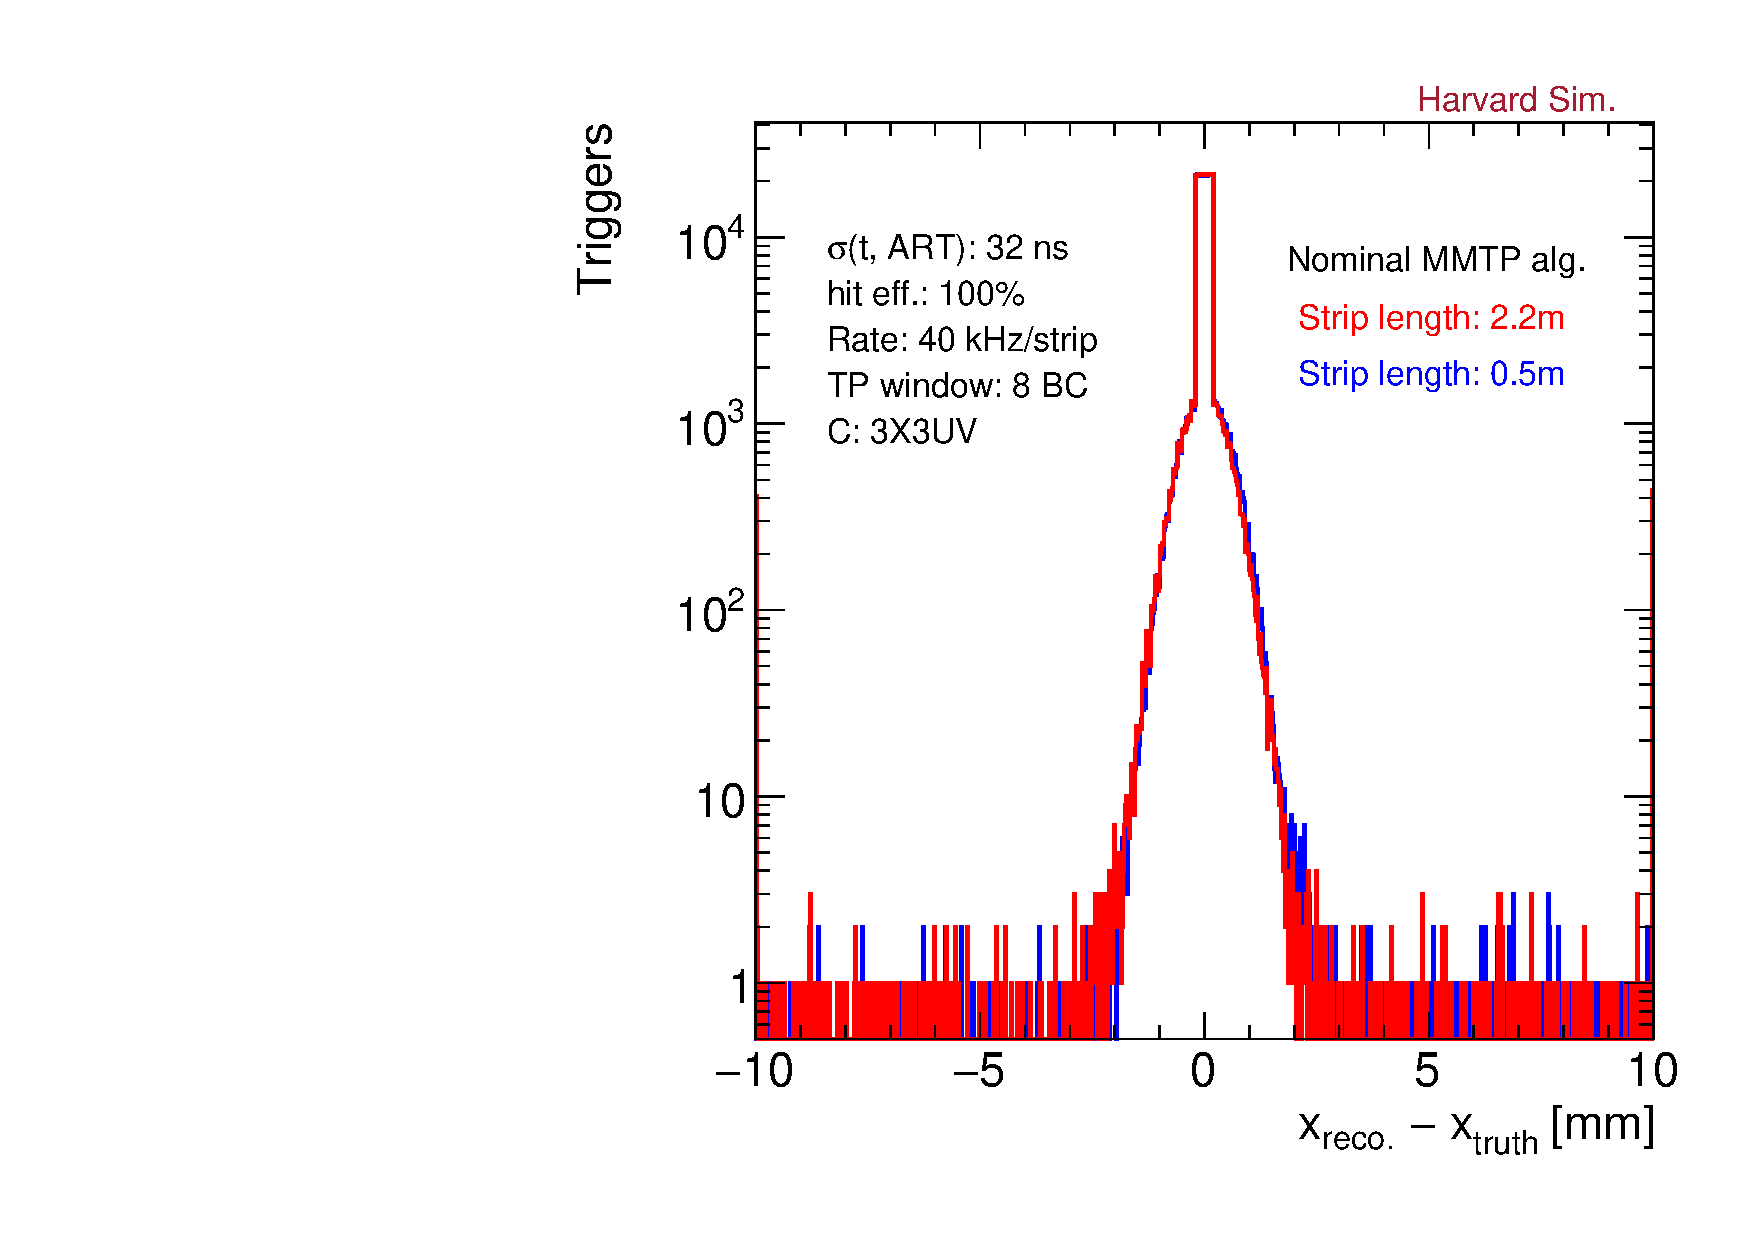
\includegraphics[width=0.48\textwidth]{figures/xres_old.pdf}
    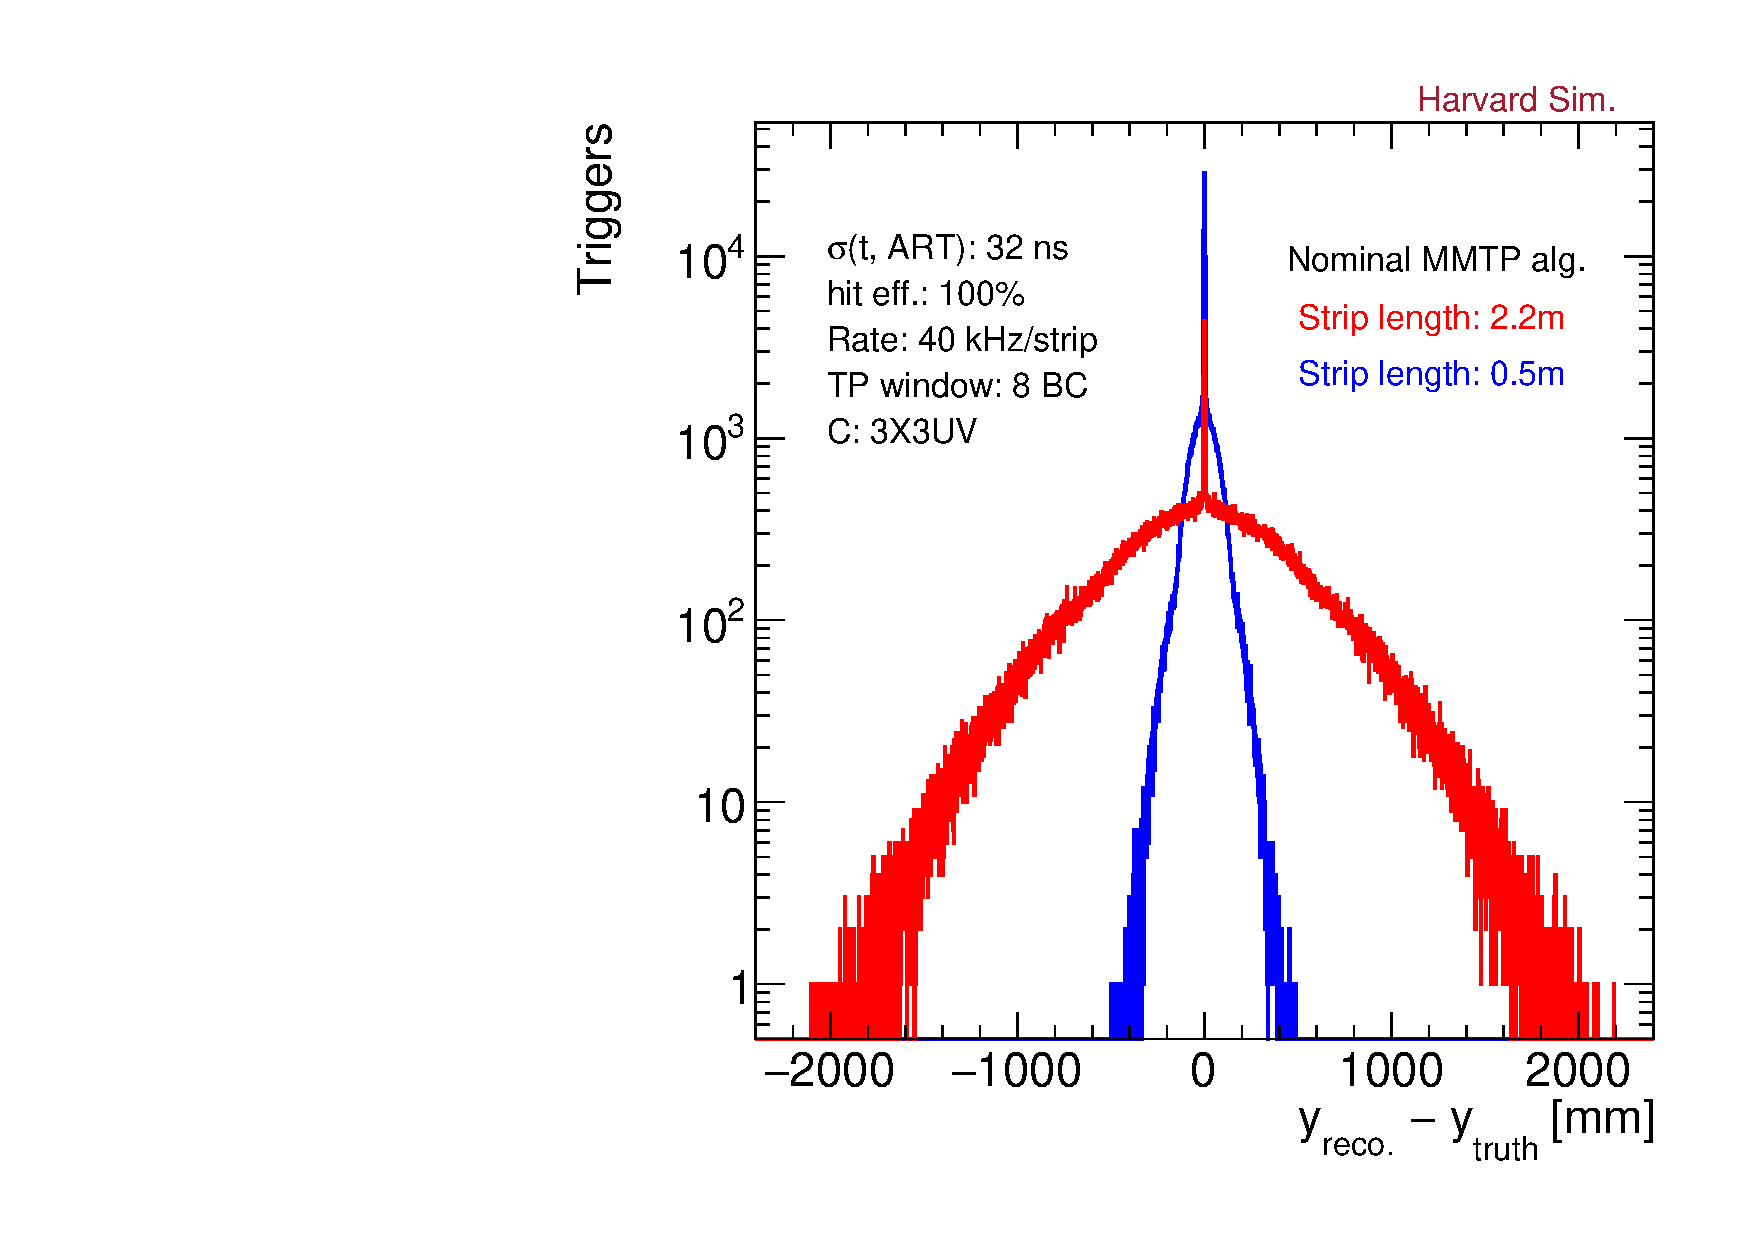
\includegraphics[width=0.48\textwidth]{figures/yres_old.pdf}
    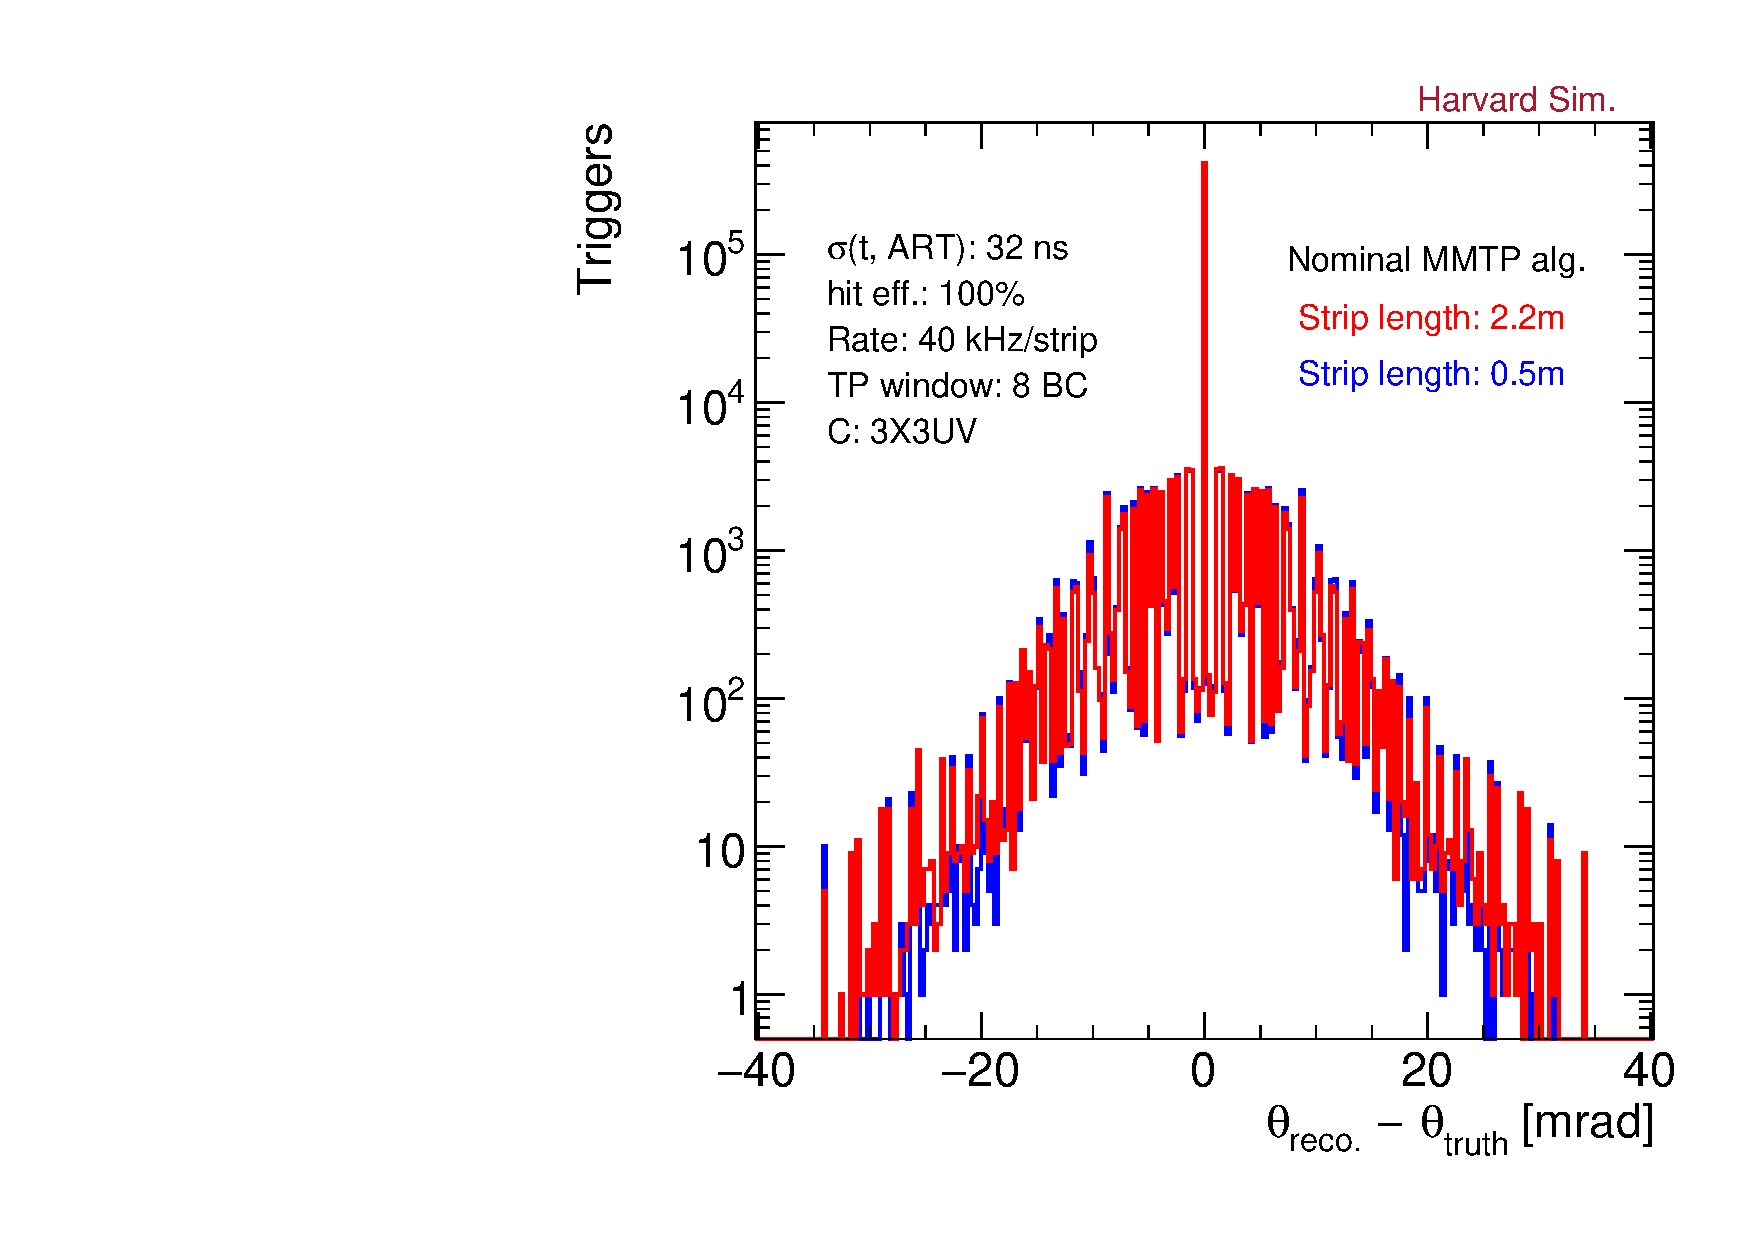
\includegraphics[width=0.48\textwidth]{figures/mres_old.pdf}
  \end{center}
  \vspace{-10pt}
  \caption{Distribution of $x_\text{reco.} - x_\text{truth}$ (top, left), $y_\text{reco.} - y_\text{truth}$ (top, right) and $\theta_\text{reco.} - \theta_\text{truth}$ (bottom) for the nominal MMTP algorithm with uncorrelated background at a rate of 40 kHz per strip.}
  \label{fig:resolutions_old}
\end{figure}

\section{Small stereo roads}
\label{sec:stereoroads}

Proposal and performance of small stereo roads.

\begin{figure}[!htpb]
  \begin{center}
    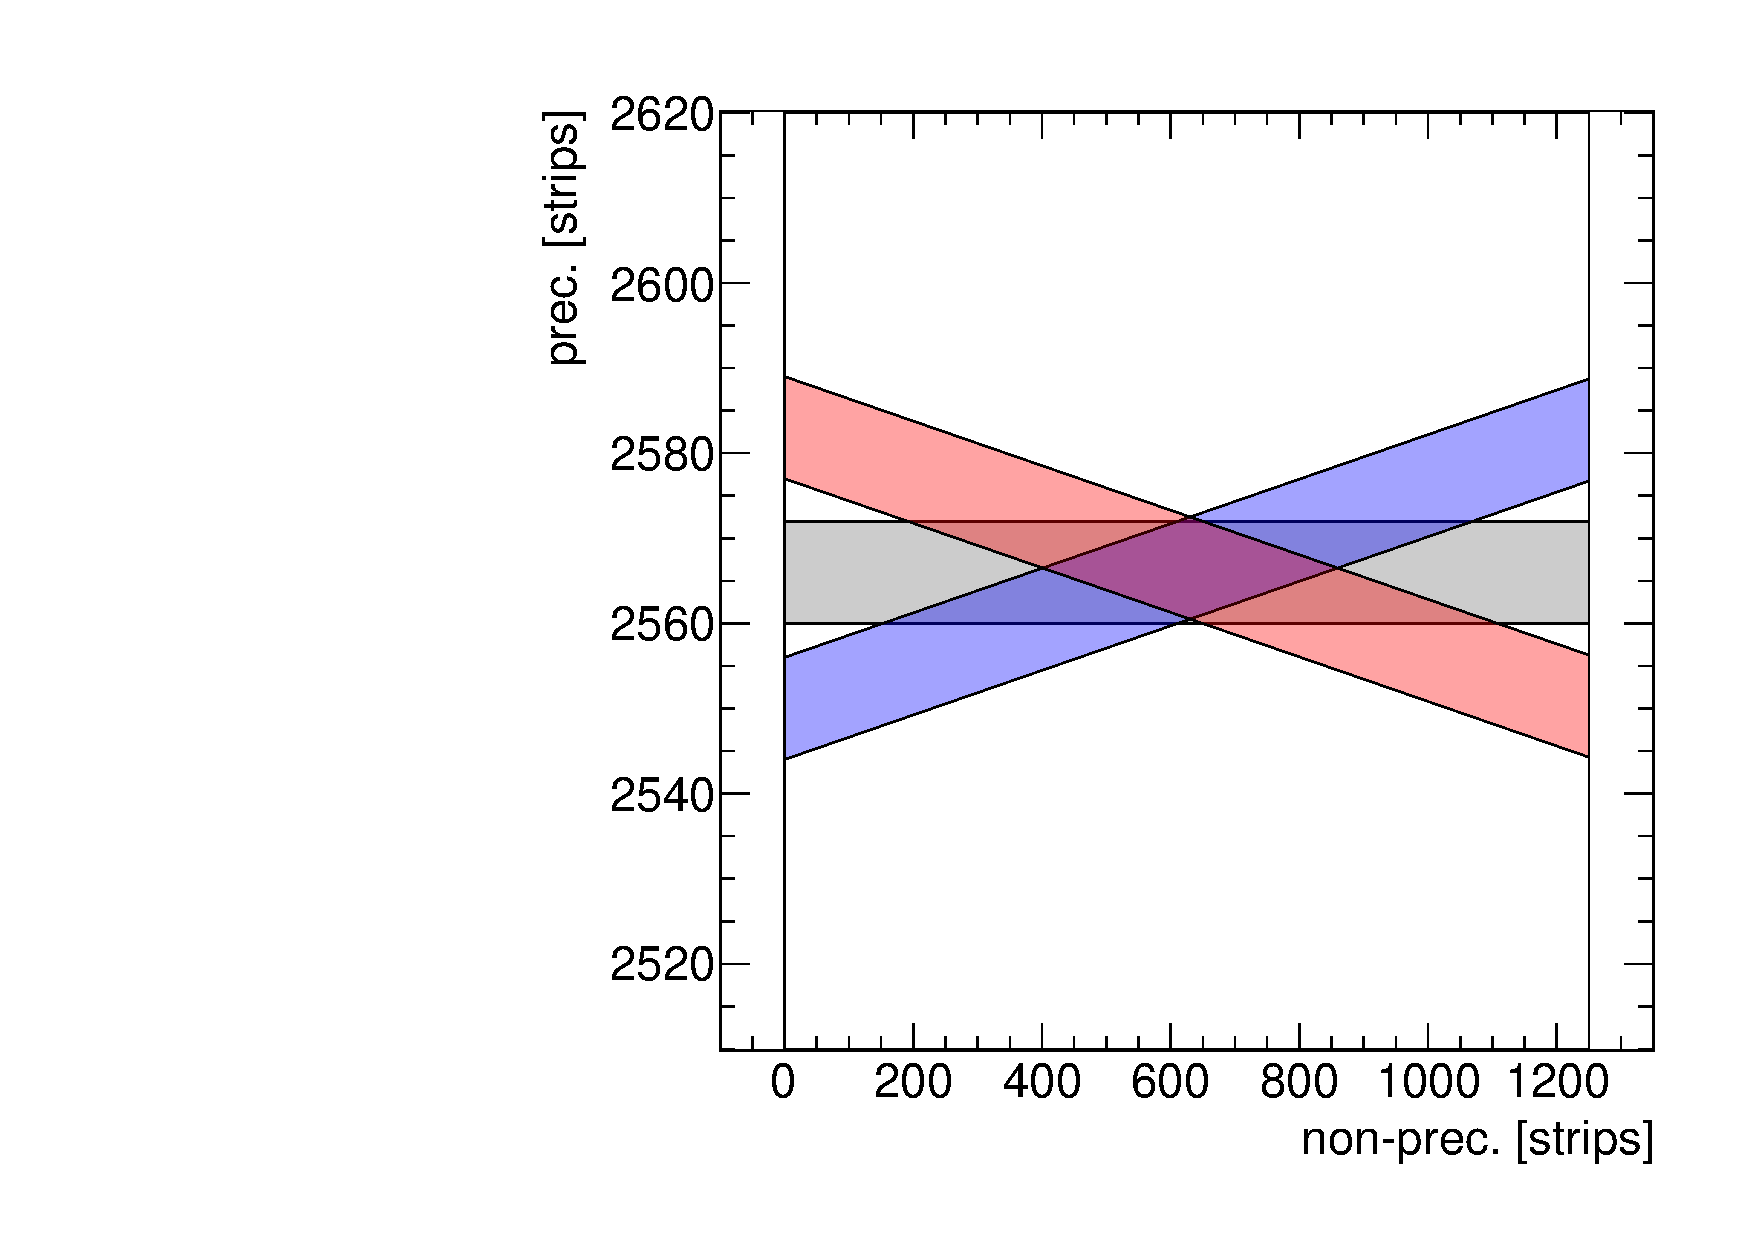
\includegraphics[width=0.48\textwidth]{figures/cartoon_roads_small_smallstereo_1.pdf}
    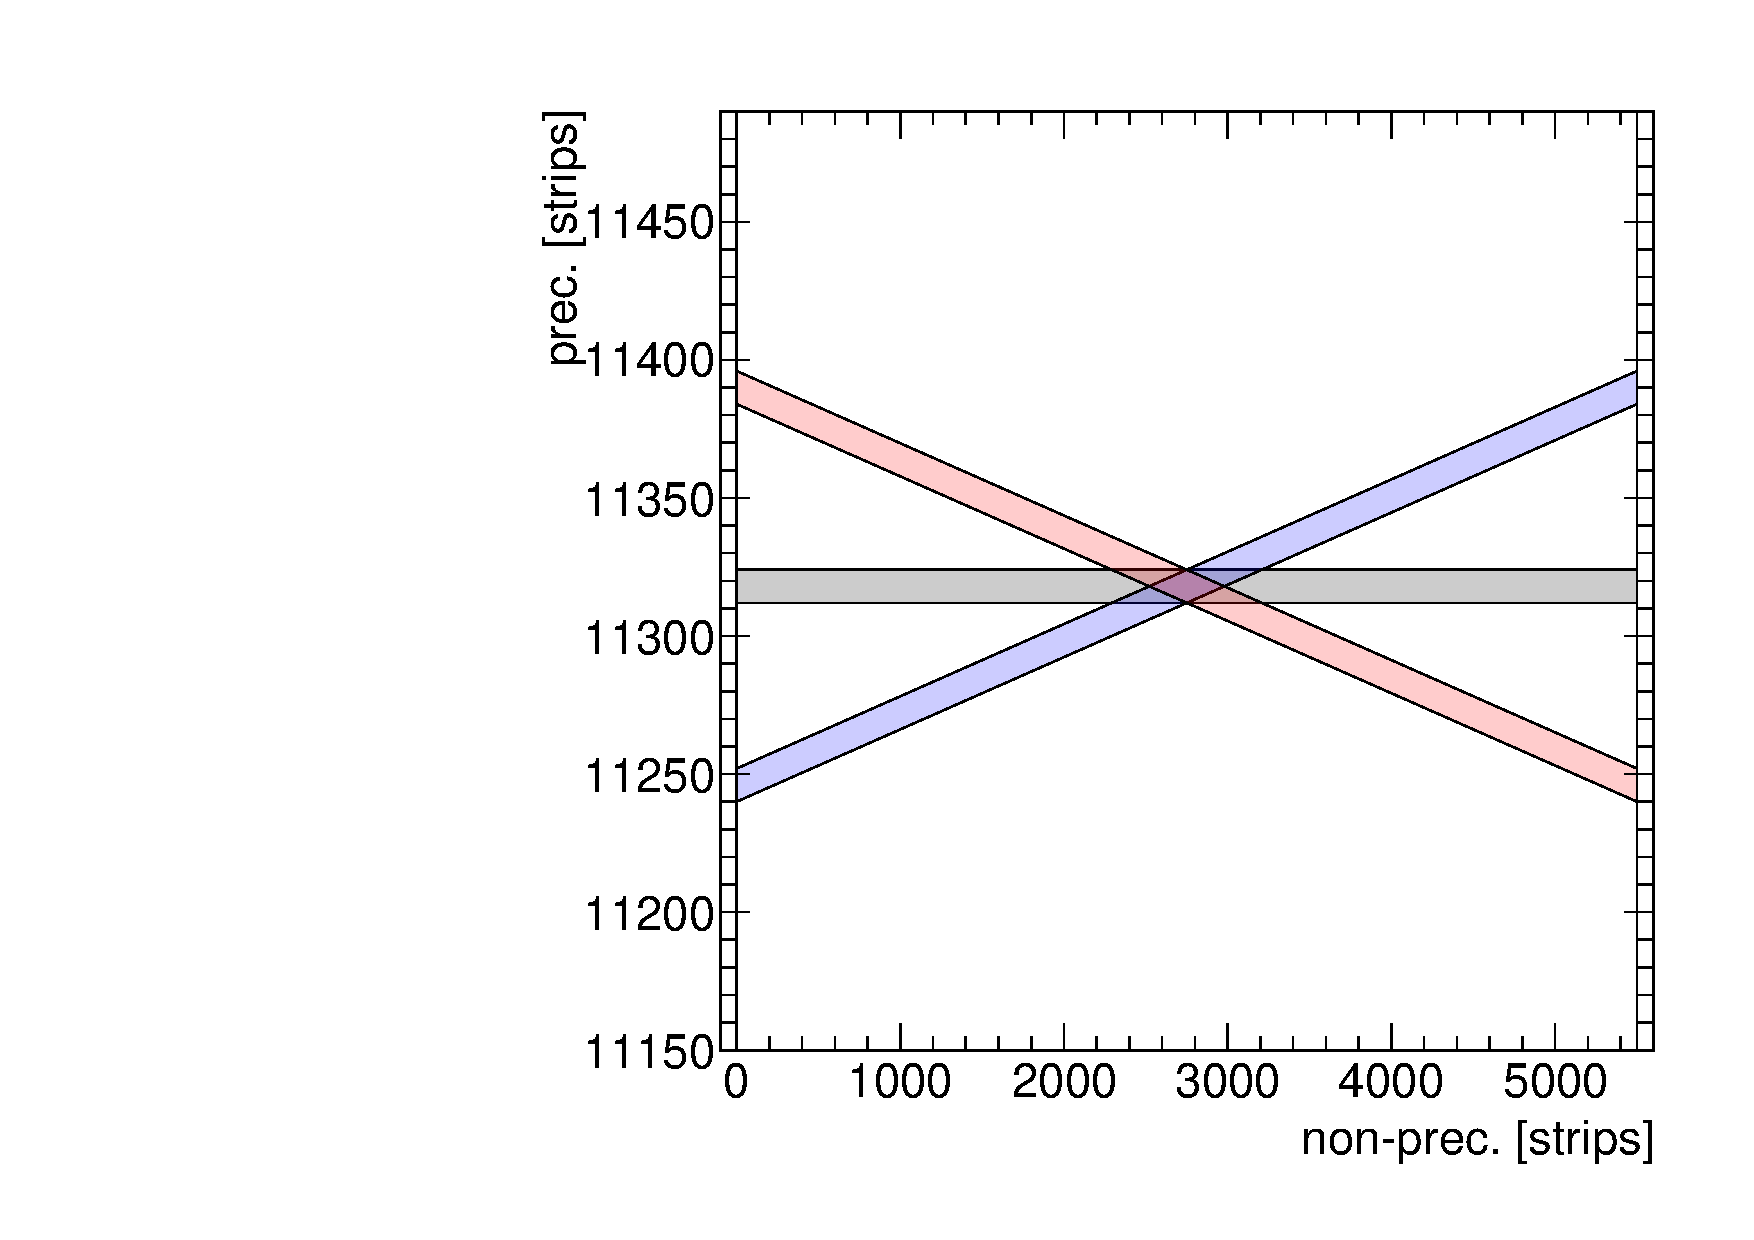
\includegraphics[width=0.48\textwidth]{figures/cartoon_roads_large_smallstereo_1.pdf}
  \end{center}
  \vspace{-10pt}
  \caption{Sketch of the road coverage of the proposed MMTP algorithm, for a small chamber closest to the beamline (left) and large chamber farthest from the beamline (right). The $X$ road is horizontal, the $U$ road is pink and slanted, and the $V$ road is blue and slanted. For ease of digestion, only one pair of $U$ and $V$ roads are shown, and they do not cover the entire $X$ road. The x-axis and y-axis are in units of strip pitches, which are 0.4 mm.}
  \label{fig:cartoon_smallroads_1}
\end{figure}

\begin{figure}[!htpb]
  \begin{center}
    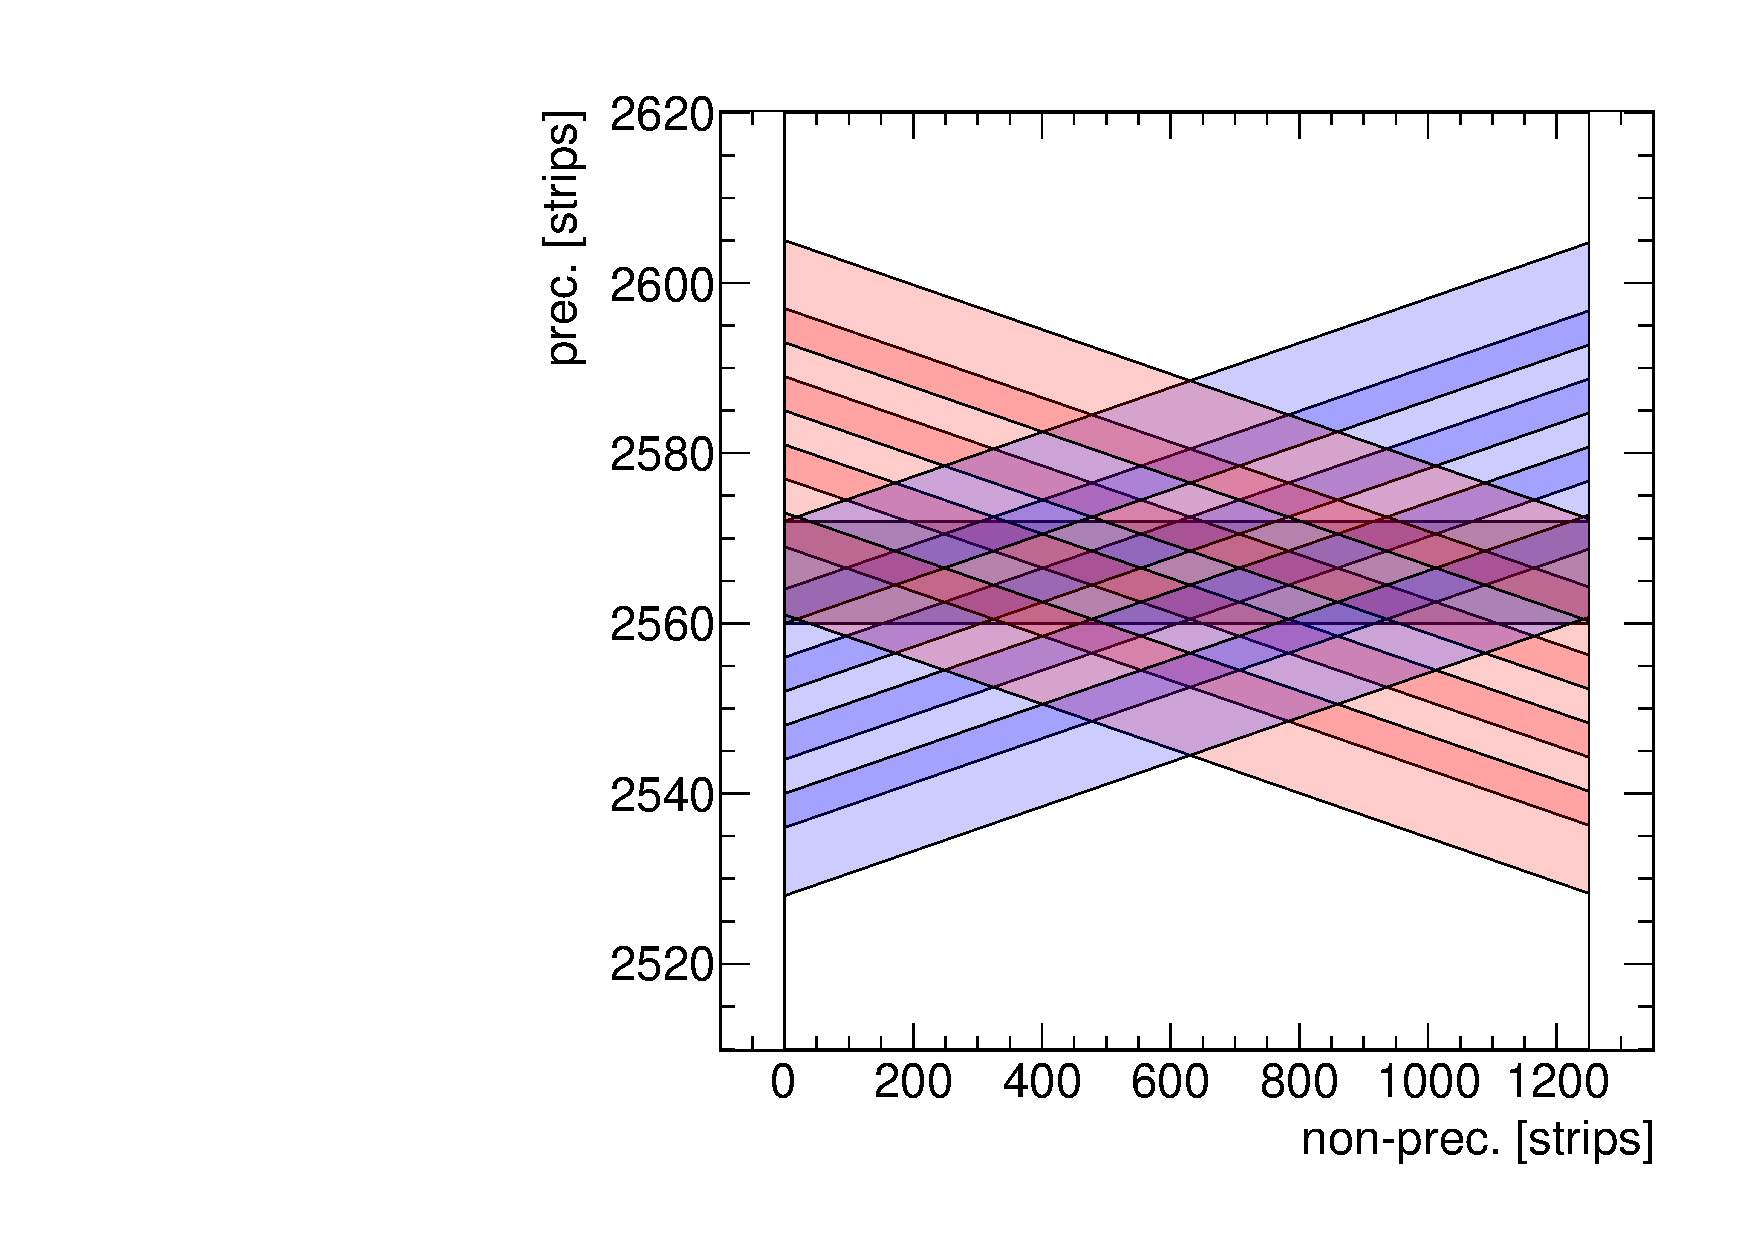
\includegraphics[width=0.48\textwidth]{figures/cartoon_roads_small_smallstereo_N.pdf}
    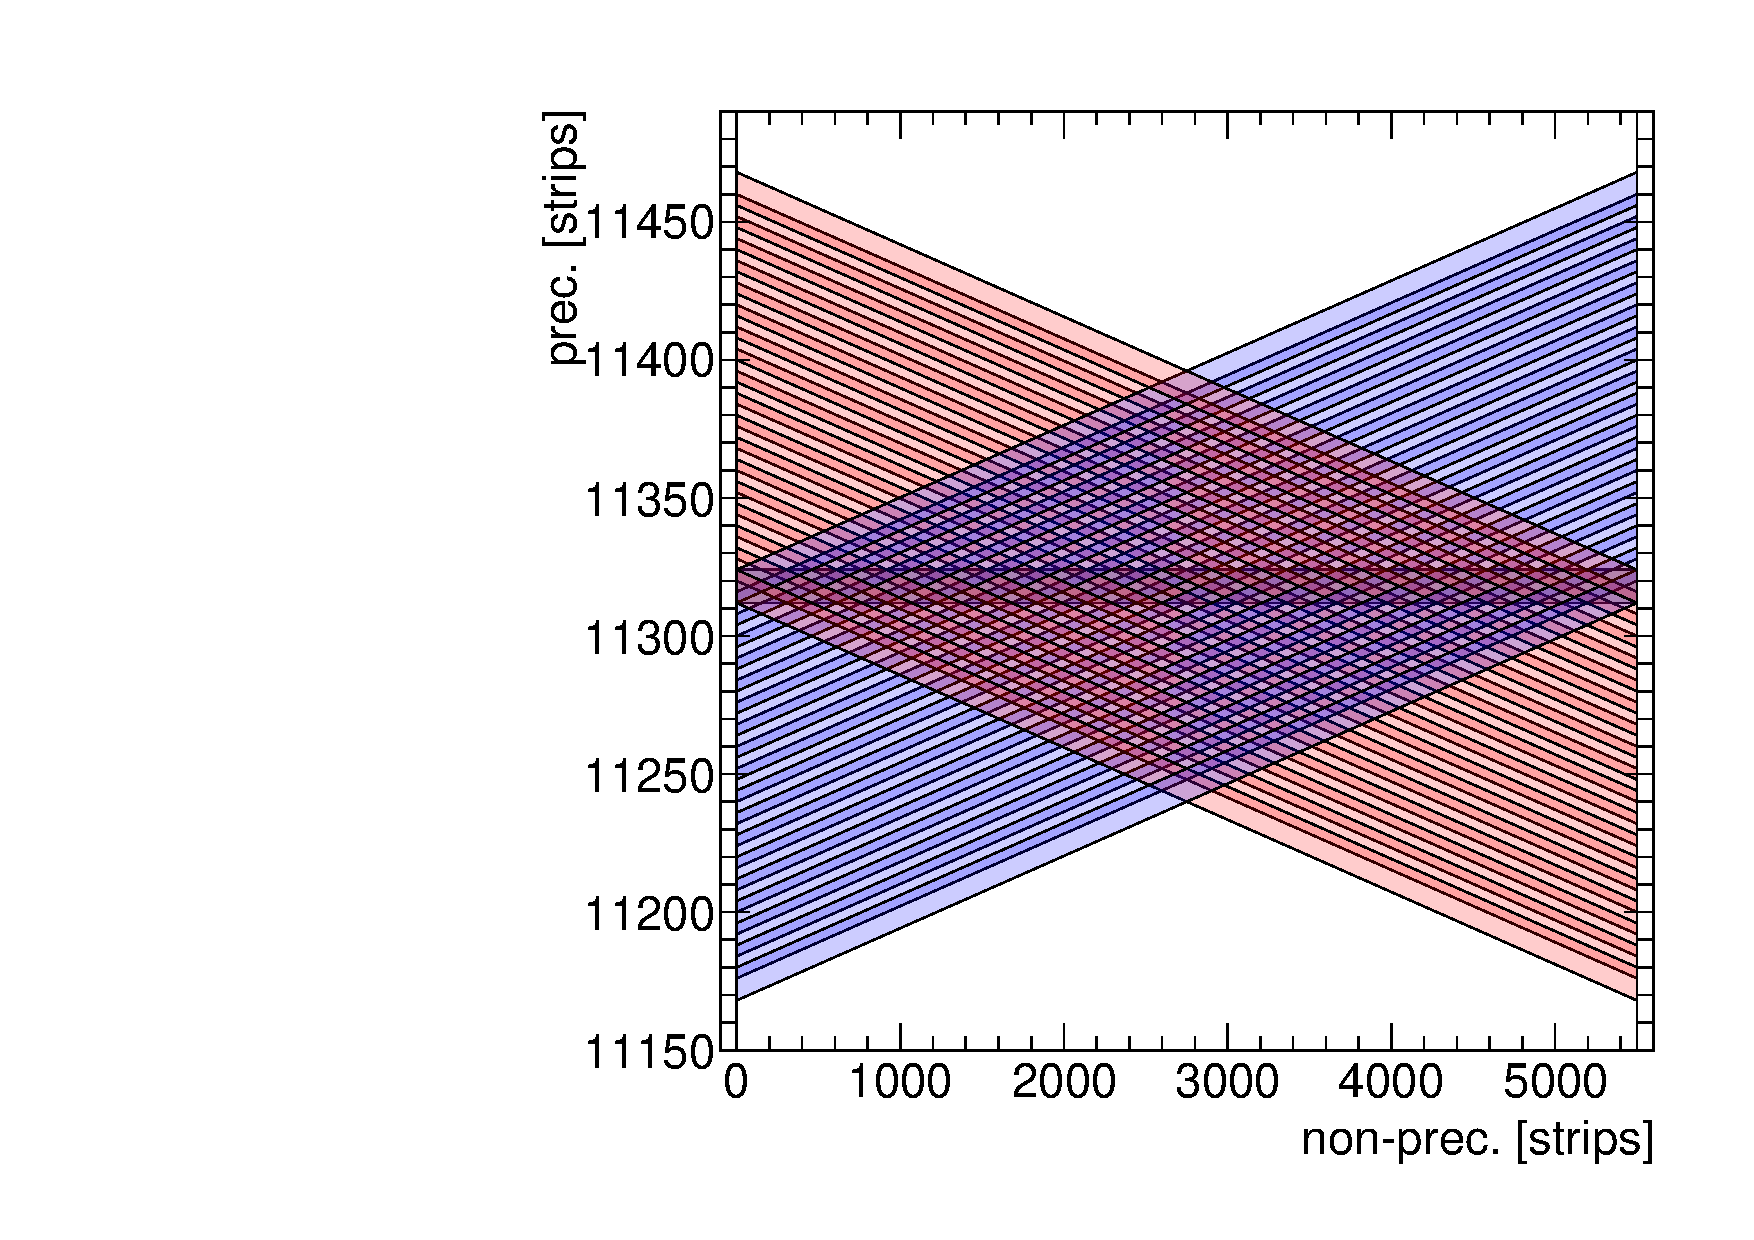
\includegraphics[width=0.48\textwidth]{figures/cartoon_roads_large_smallstereo_N.pdf}
  \end{center}
  \vspace{-10pt}
  \caption{Sketch of the road coverage of the proposed MMTP algorithm, for a small chamber closest to the beamline (left) and large chamber farthest from the beamline (right). The $X$ road is horizontal, the $U$ roads are pink and slanted, and the $V$ roads are blue and slanted. The small chamber requires five pairs of $U$ and $V$ roads to cover one $X$ road, and the large chamber requires 19. The x-axis and y-axis are in units of strip pitches, which are 0.4 mm.}
  \label{fig:cartoon_smallroads_N}
\end{figure}

\begin{figure}[!htpb]
  \begin{center}
    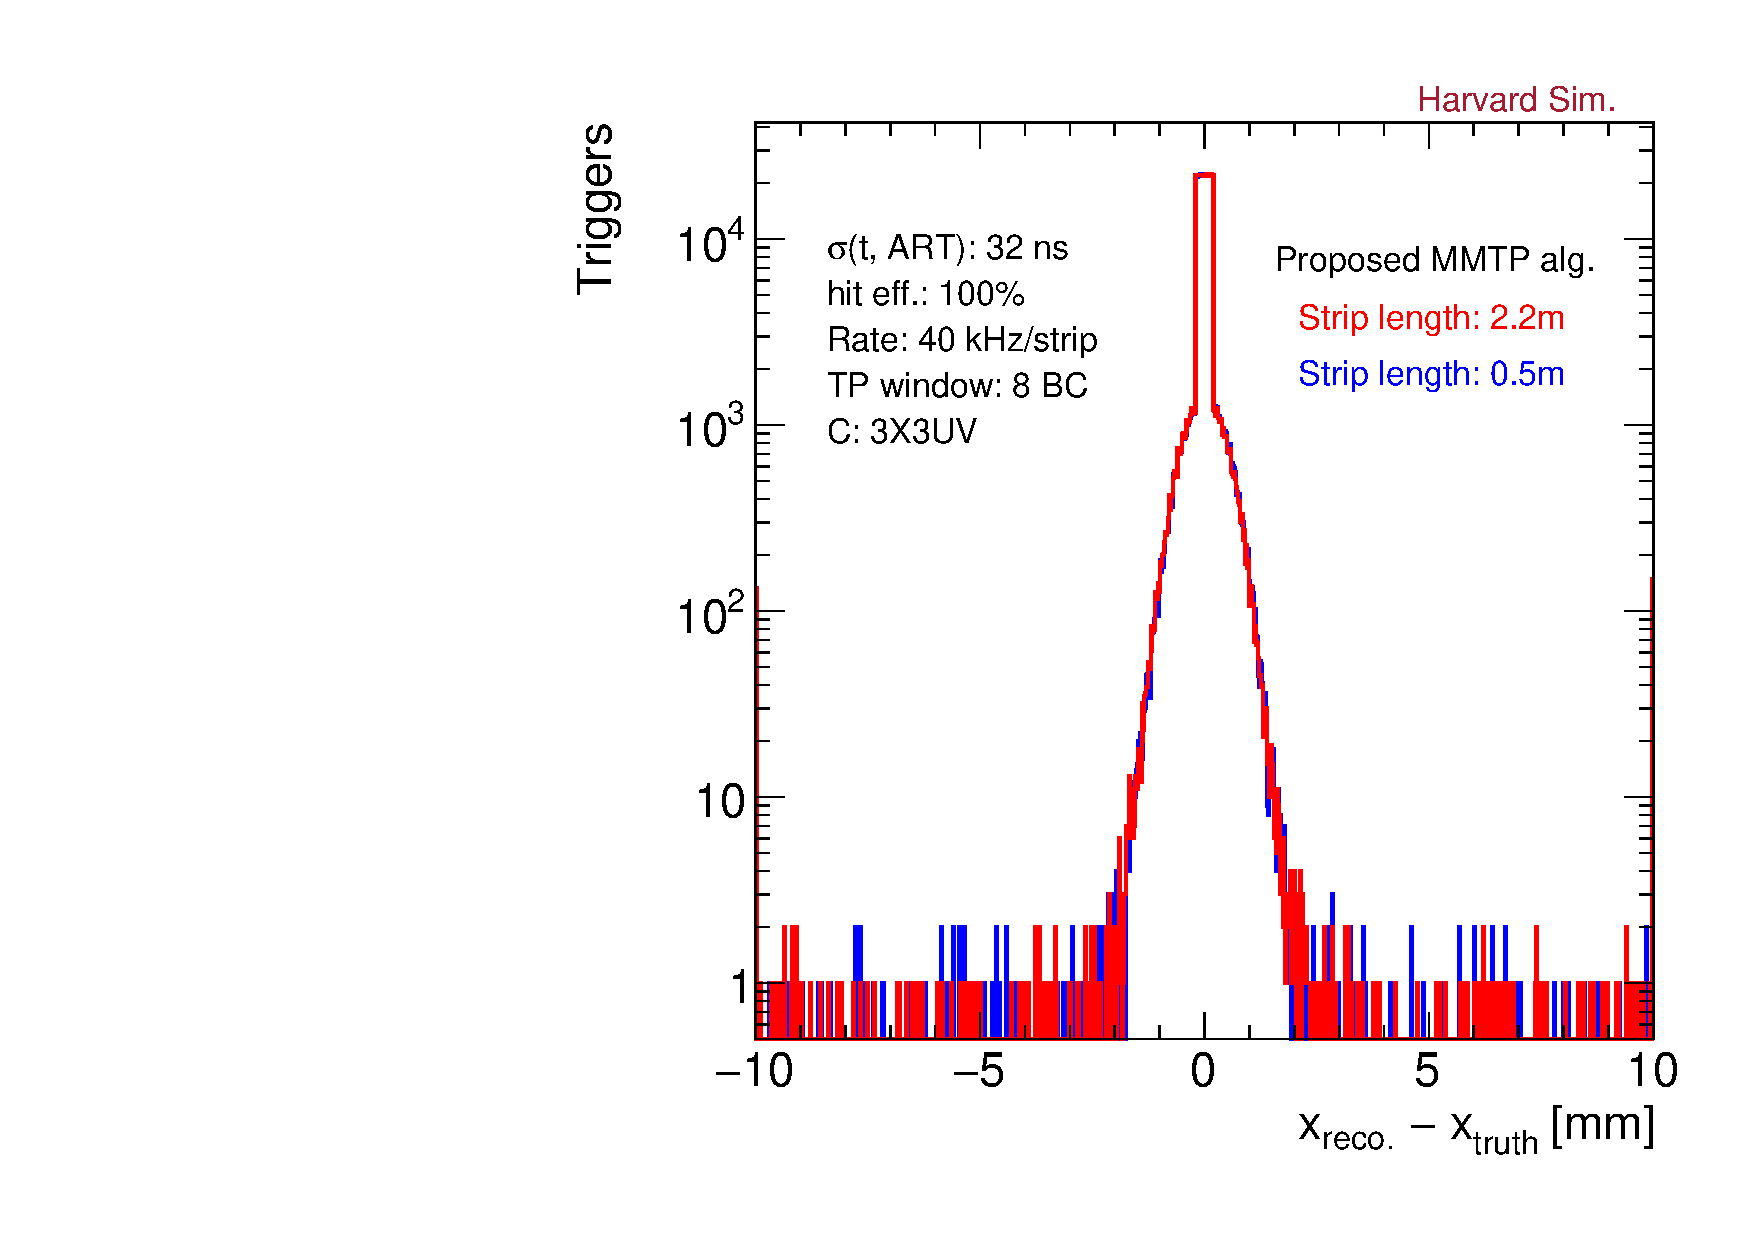
\includegraphics[width=0.48\textwidth]{figures/xres_new.pdf}
    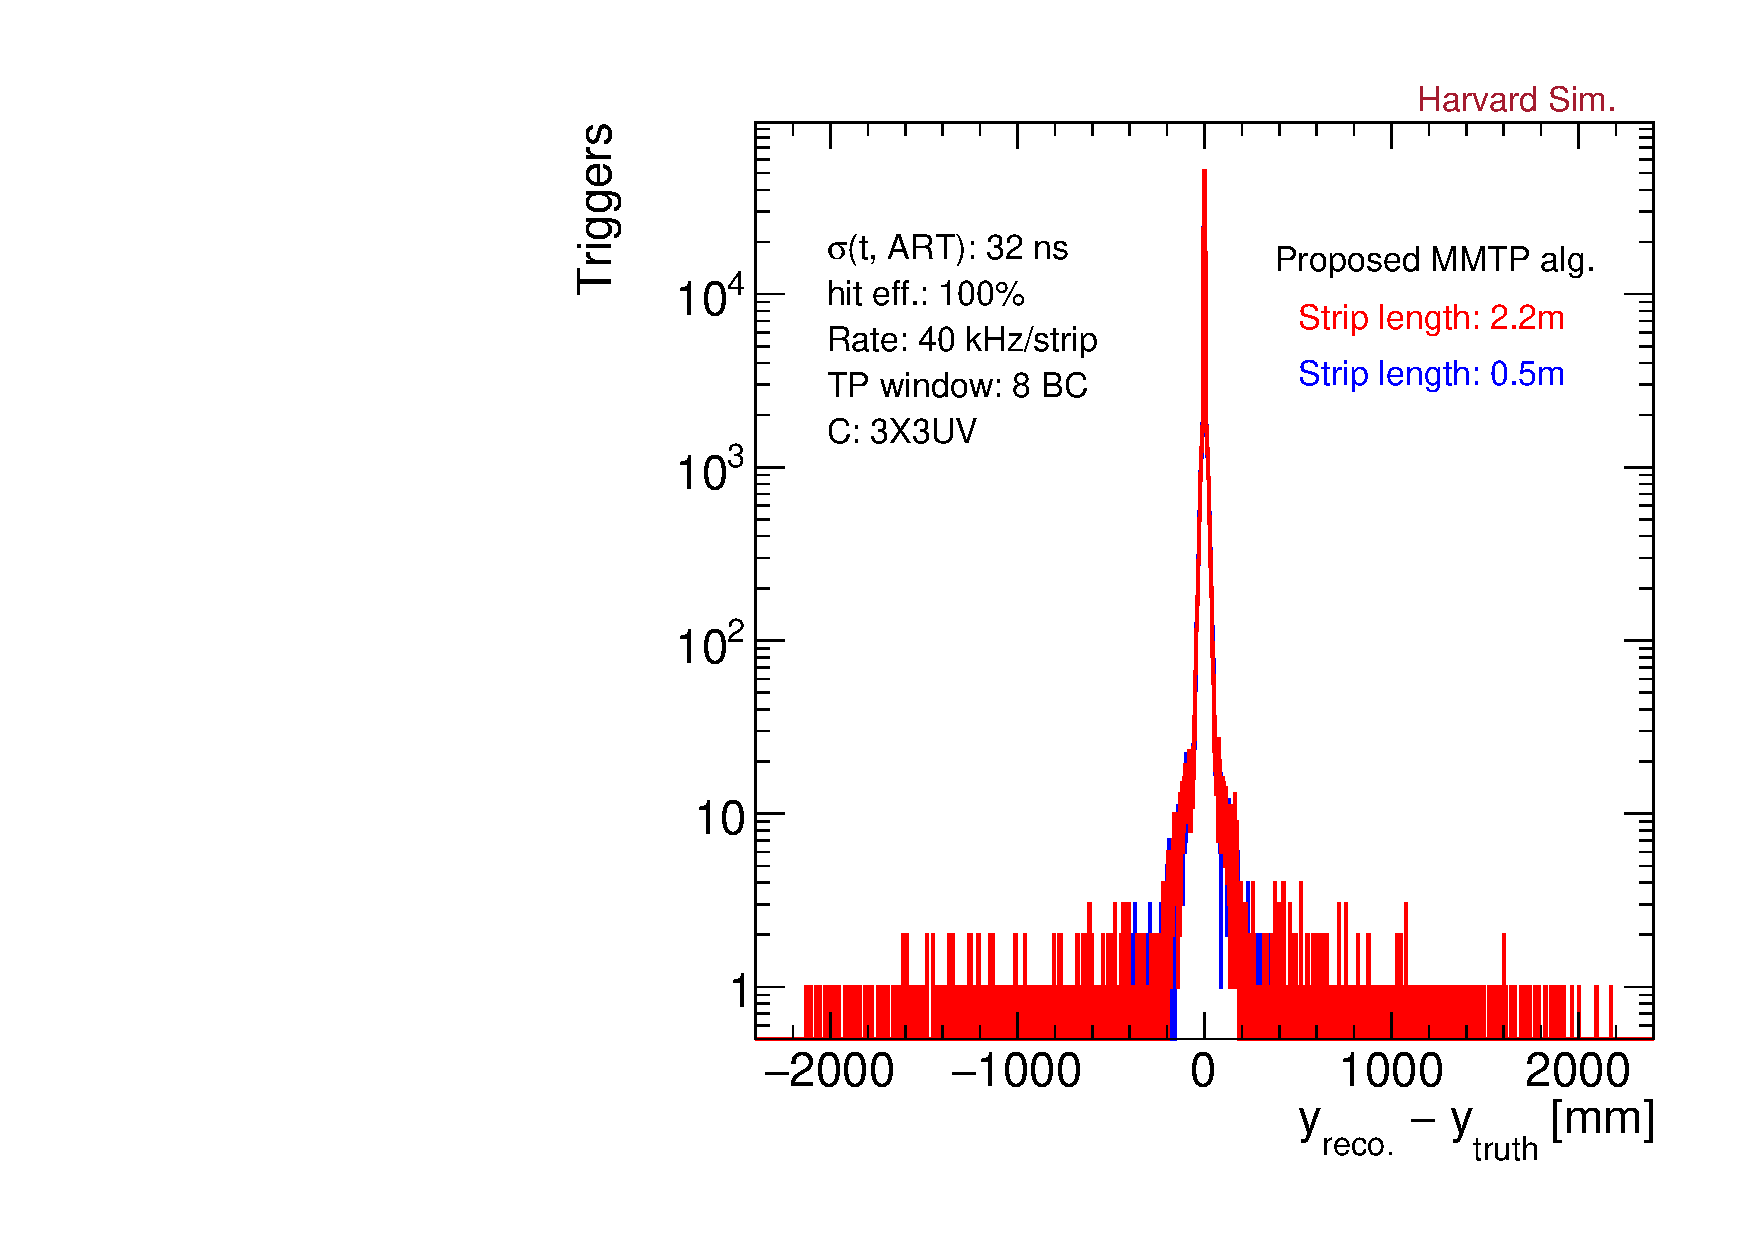
\includegraphics[width=0.48\textwidth]{figures/yres_new.pdf}
    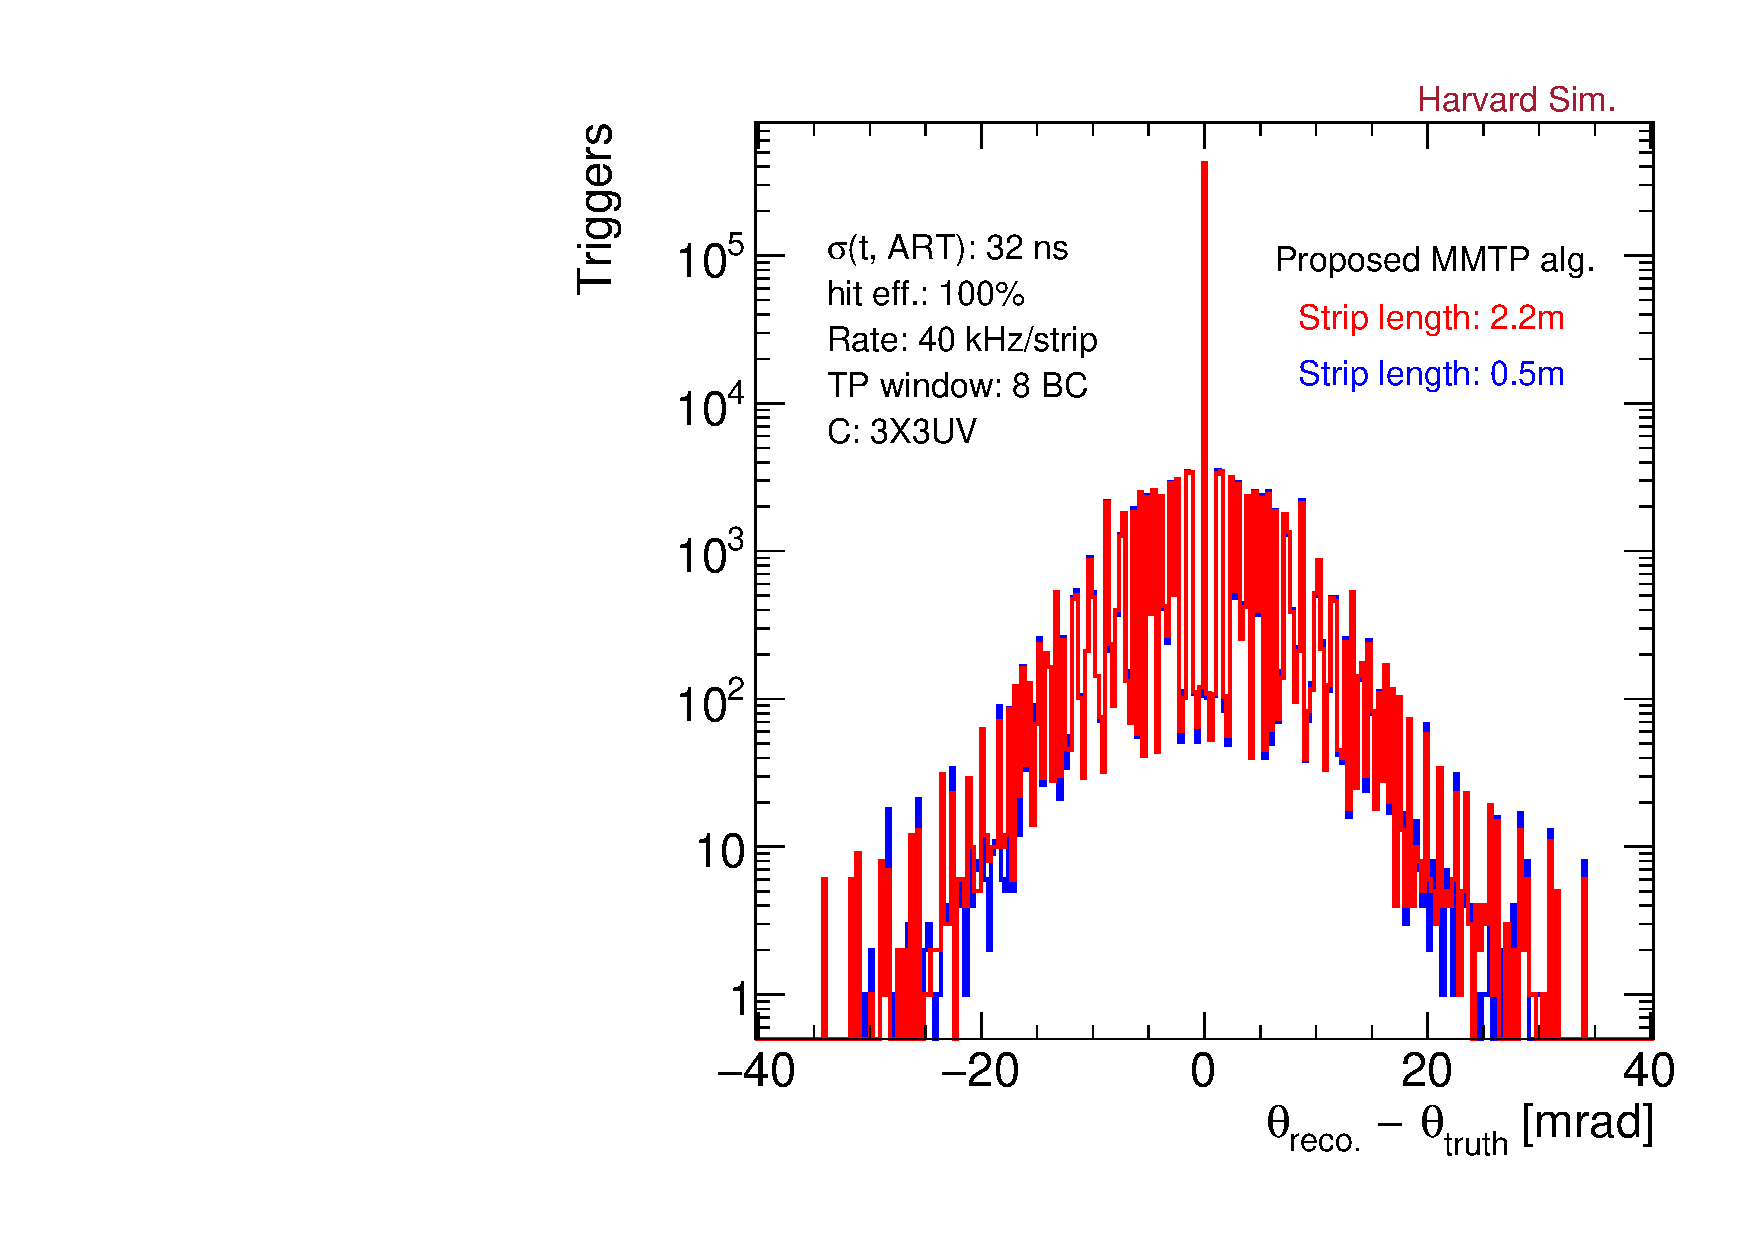
\includegraphics[width=0.48\textwidth]{figures/mres_new.pdf}
  \end{center}
  \vspace{-10pt}
  \caption{Distribution of $x_\text{reco.} - x_\text{truth}$ (top, left), $y_\text{reco.} - y_\text{truth}$ (top, right) and $\theta_\text{reco.} - \theta_\text{truth}$ (bottom) for the nominal MMTP algorithm with uncorrelated background at a rate of 40 kHz per strip.}
  \label{fig:resolutions_old}
\end{figure}

\begin{figure}[!htpb]
  \begin{center}
    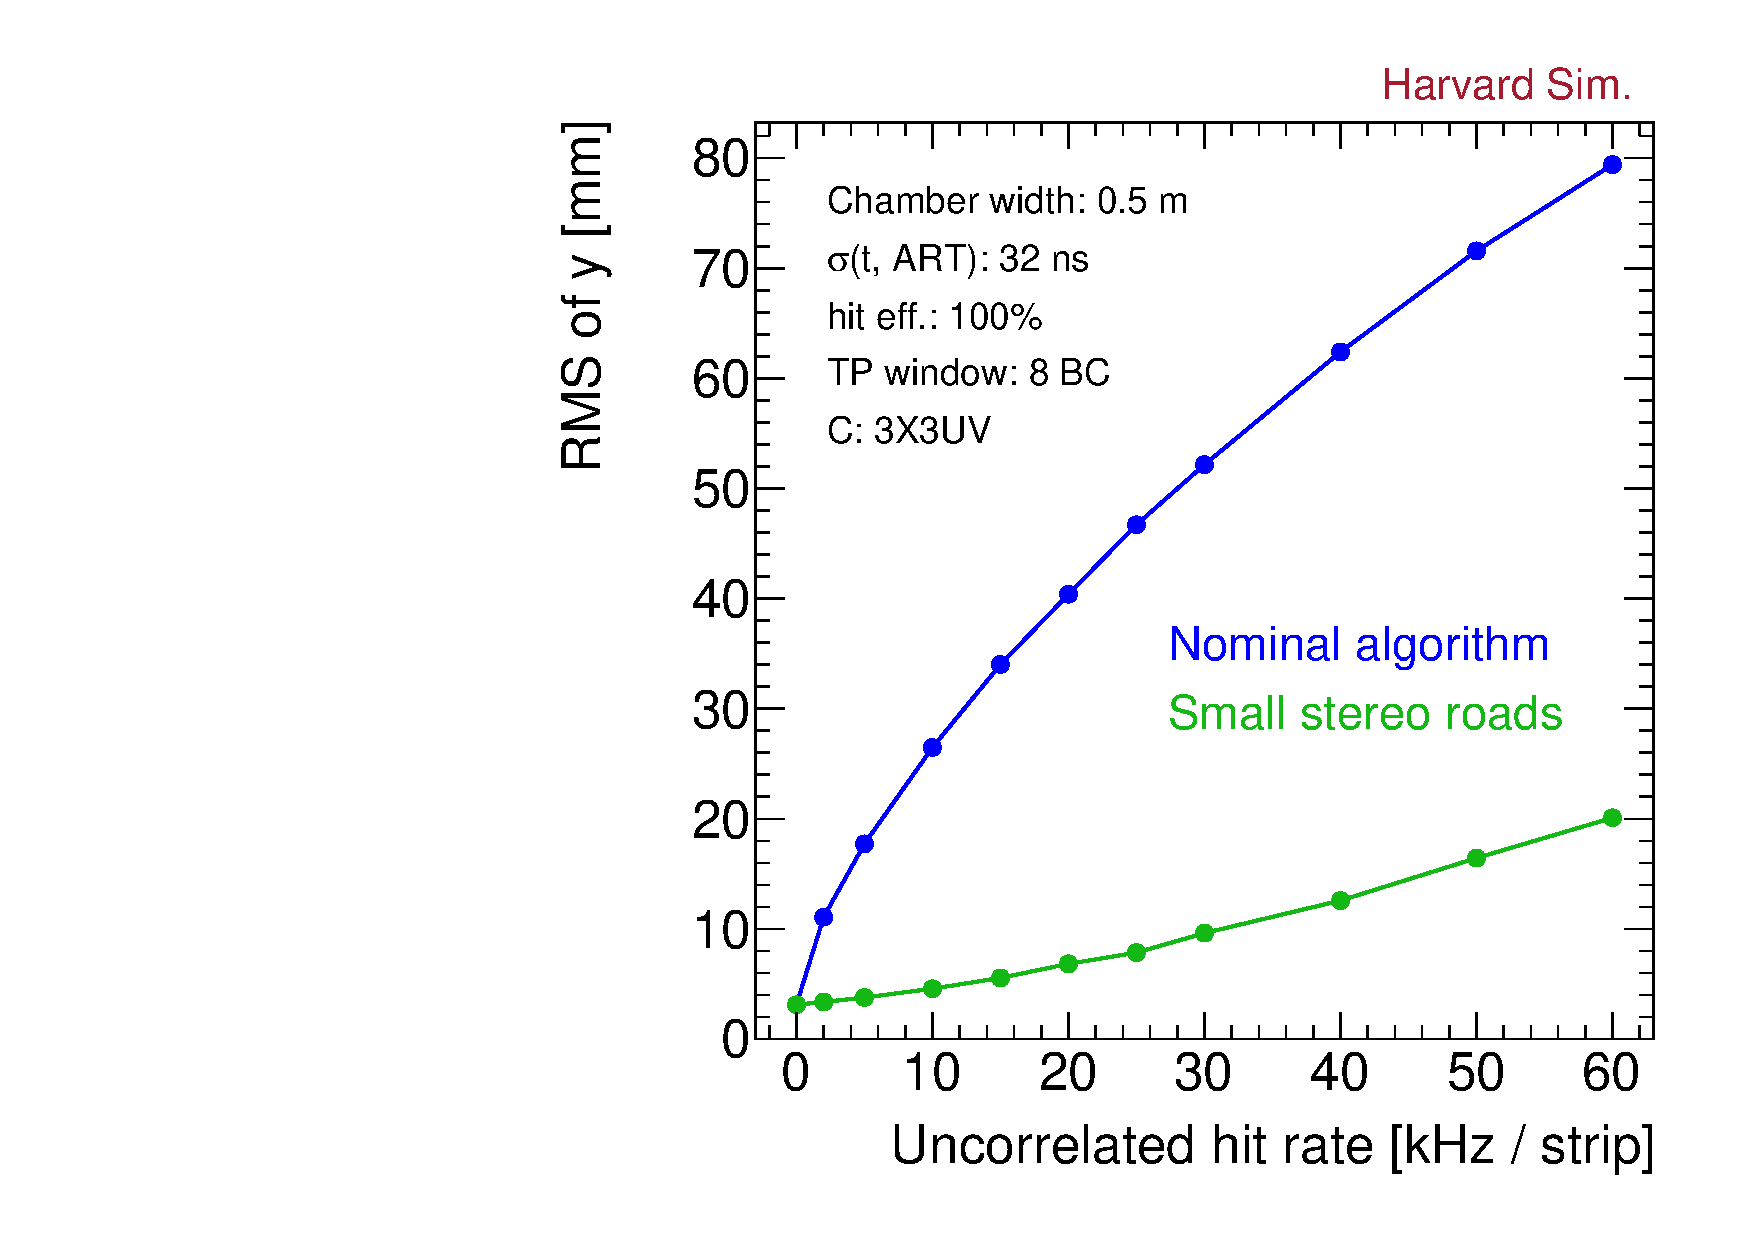
\includegraphics[width=0.48\textwidth]{figures/rms_y_small_vs_rate.pdf}
    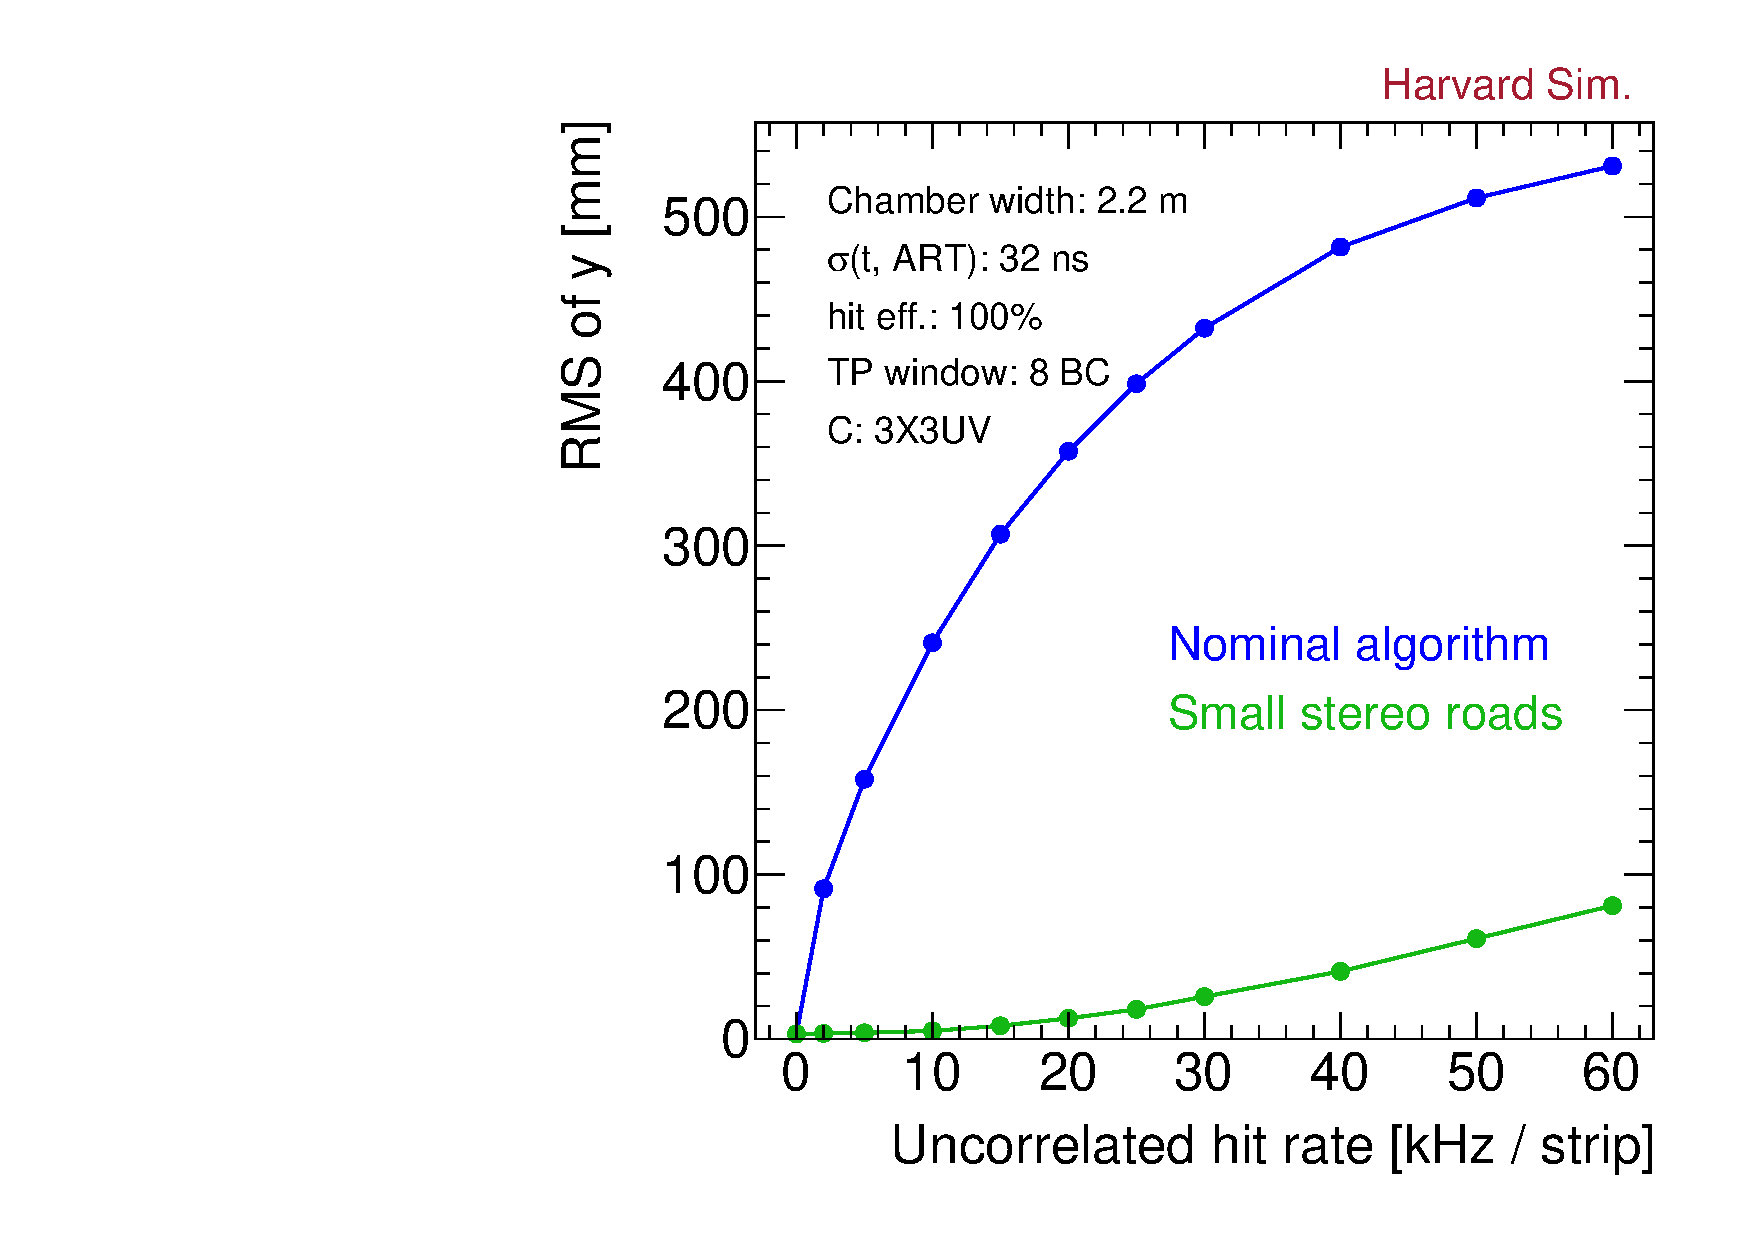
\includegraphics[width=0.48\textwidth]{figures/rms_y_large_vs_rate.pdf}
  \end{center}
  \vspace{-10pt}
  \caption{RMS of $y_\text{reco.} - y_\text{truth}$ for a small chamber of width 0.5m (left) and large chamber of width 2.2m (right) as a function of uncorrelated background rate. The RMS is calculated in the $3\sigma$ (99.7\%) range of the distribution.}
  \label{fig:rms_vs_rate}
\end{figure}

\begin{figure}[!htpb]
  \begin{center}
    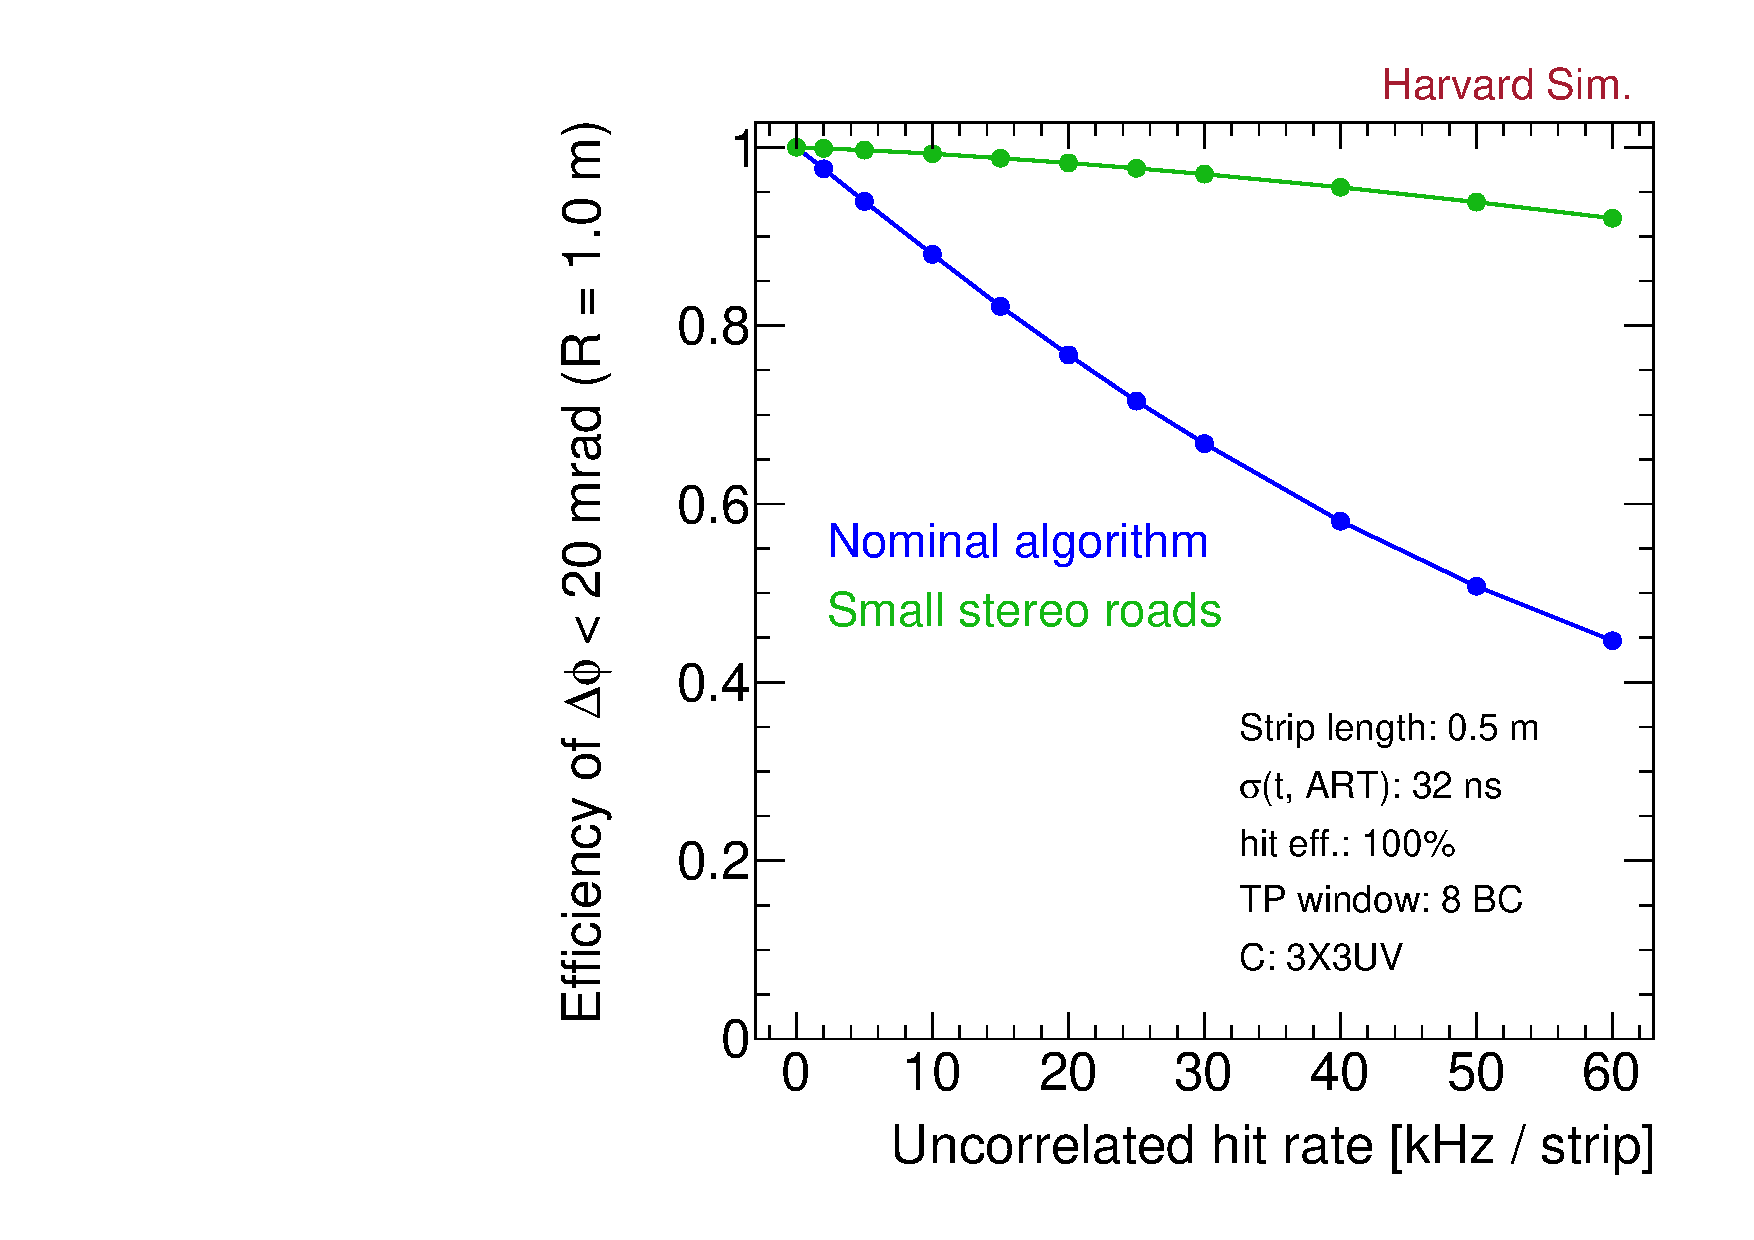
\includegraphics[width=0.48\textwidth]{figures/eff_phi_small_vs_rate.pdf}
    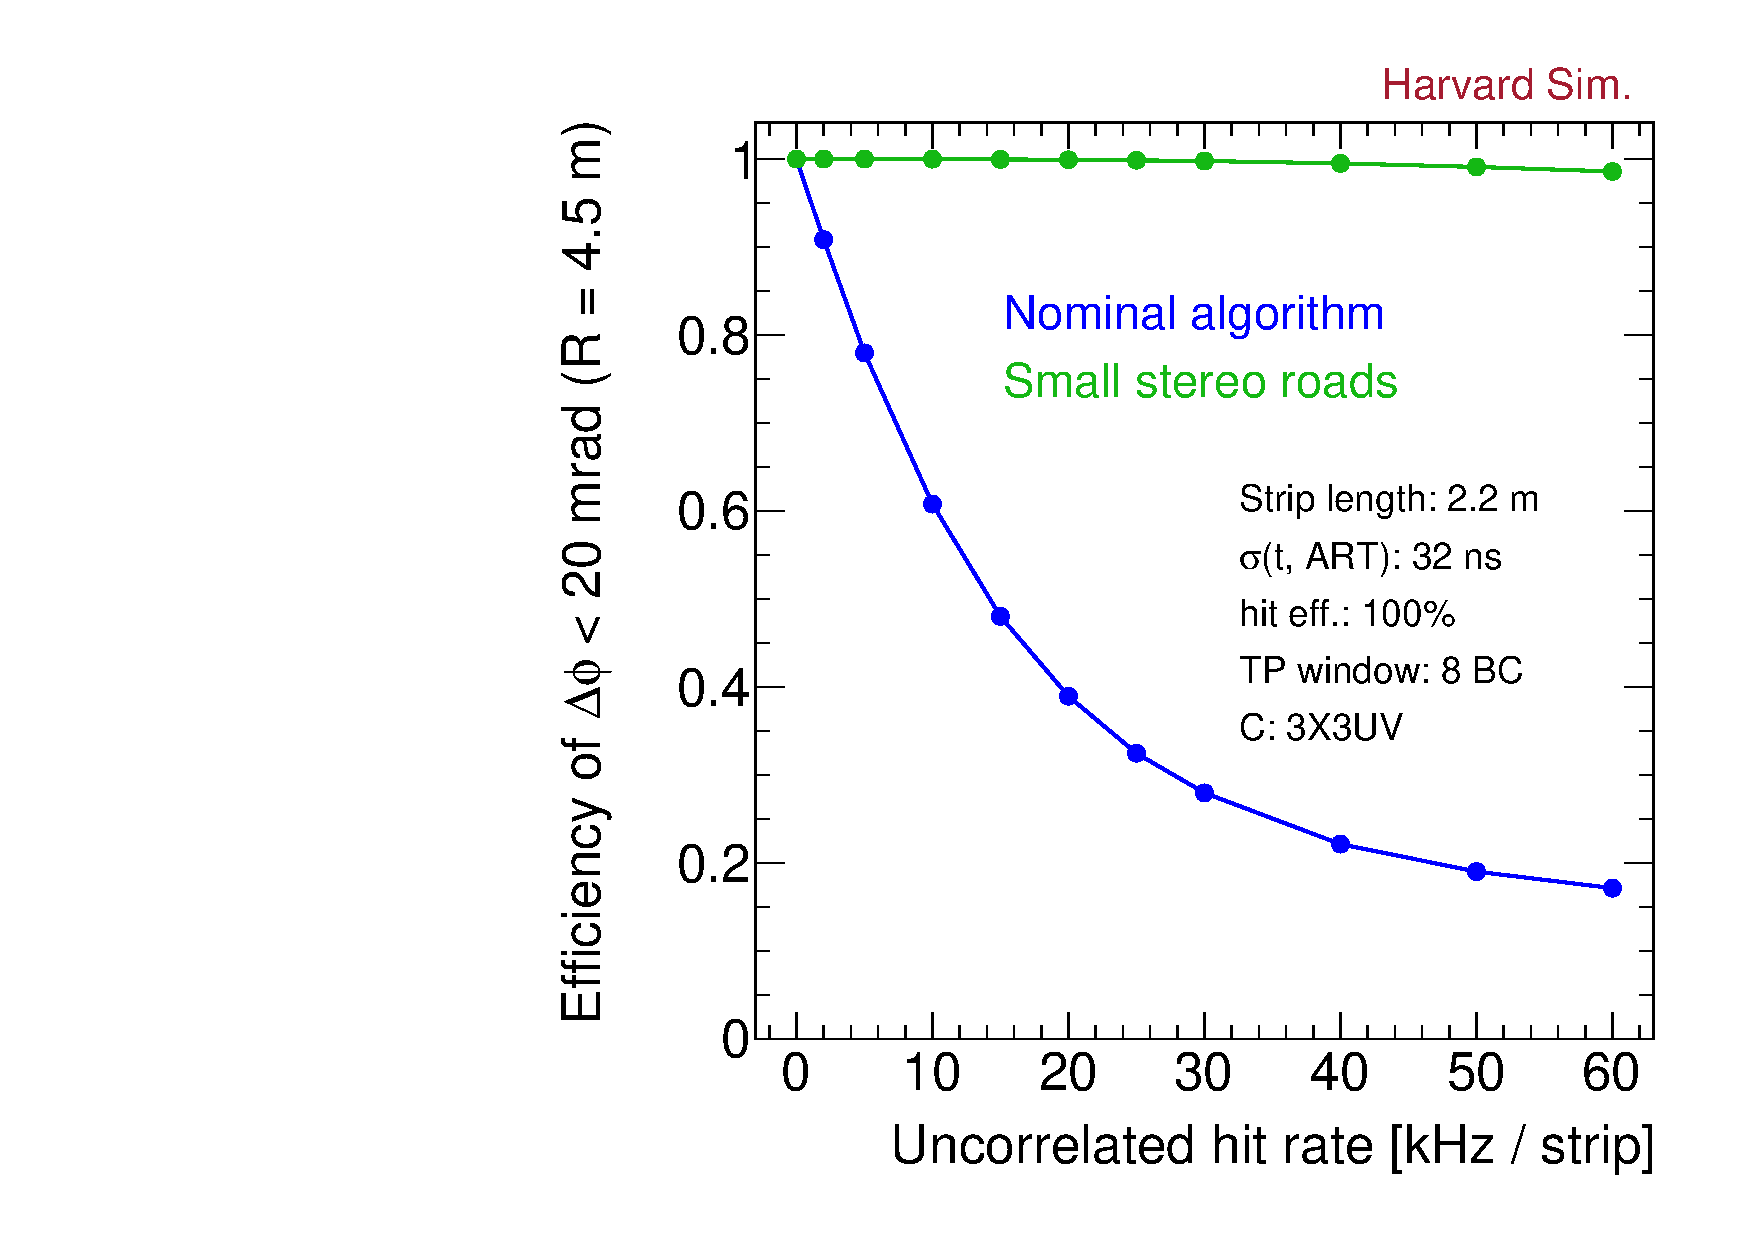
\includegraphics[width=0.48\textwidth]{figures/eff_phi_large_vs_rate.pdf}
  \end{center}
  \vspace{-10pt}
  \caption{Efficiency of $\phi_\text{reco.} - \phi_\text{truth} < 20$ mrad for a small chamber (left) and large chamber (right). $\phi_\text{reco.}-\phi_\text{truth}$ is calculated as $\frac{y_\text{reco.} - y_\text{truth}}{R}$, where $R$ is the distance from the beamline. $R$ is taken to be 1m for the small chamber and 4.5m for the large chamber.}
  \label{fig:eff_vs_rate}
\end{figure}


\section{Hardware resources}
\label{sec:fpga}

FPGA resources.



\section{Conclusion}
\label{sec:conclusion}

Conclusion.




\clearpage

\begin{thebibliography}{99}
\label{bibliography}
\setlength{\itemsep}{1.5pt plus 2.0pt minus 1.4pt}
\setlength{\parsep}{0pt}
\setlength{\parskip}{0pt}
\vspace{-6pt}
\bibitem{nswtdr} ATLAS New Small Wheel Technical Design Report. \href{http://cds.cern.ch/record/1552862}{\color{blue}\underline{ATLAS-TDR-020}}.
 \href{https://cds.cern.ch/record/2272355}{\color{blue}\underline{ATL-COM-MUON-2017-036}}.
\bibitem{noisy} P.~Giromini {\it et al,} Performance of a Micromegs octuplet in the time  of noise.
 \href{https://cds.cern.ch/record/2277316}{\color{blue}\underline{ATL-COM-MUON-2017-036}}.
\bibitem{noiseless} P.~Giromini  {\it et al,} Performance of a Micromegs octuplet after removing the major cause of noise.
 \href{https://cds.cern.ch/record/2277316}{\color{blue}\underline{ATL-COM-MUON-2017-040}}.
\bibitem{mmfe8} \url{https://twiki.cern.ch/twiki/bin/viewauth/Atlas/NewSmallWheel}.
\bibitem{addc} \url{https://twiki.cern.ch/twiki/pub/Atlas/February_2015_design_reviews/ADDC_document_for_2015_Feb_NSW_review_v1.0.pdf}.
\bibitem{brian} B.~Clark {\it et al,} An Algorithm for Micromegas Segment
 Reconstruction in the Level-1 Trigger of the New Small Wheel. \href{https://cds.cern.ch/record/1706160}{\color{blue}\underline{ATL-COM-UPGRADE-2014-012}}.
\bibitem{steve} S.~Chan et. al. Micromegas Trigger Processor Algorithm Performance in Nominal, Misaligned, and Misalignment
 Corrected Conditions. \href{https://cds.cern.ch/record/2113121}{\color{blue}\underline{ATL-COM-UPGRADE-2015-033}}.
\bibitem{oldart} K.~DiPetrillo  {it et al,} ATL-COM-MUON-2014-069.
\bibitem{koki} Simulation of the ATLAS New Small Wheel (NSW) System
 \href{http://cds.cern.ch/record/2265067}{\color{blue}\underline{ATL-MUON-SLIDE-2017-248}}.
\bibitem{phase2} ATLAS Muon Spectrometer Phase-II Upgrade Technical Design Report. \href{https://cds.cern.ch/record/2270169/}{\color{blue}\underline{ATL-COM-MUON-2017-033}}.
\end{thebibliography}










\end{document} 

